\documentclass[a4paper,11pt]{article}
%\usepackage{jinstpub} % for details on the use of the package, please see the JINST-author-manual
\usepackage{lineno}
\usepackage{siunitx}
\usepackage{hyperref}
\linenumbers
\usepackage[backend=bibtex,style=ieee]{biblatex}
\addbibresource{biblio.bib}
\usepackage{url}
\usepackage{graphicx}
\usepackage{amsmath}
\usepackage{siunitx}
\usepackage[margin=1.1in]{geometry}
\usepackage[capitalise,noabbrev] {cleveref}

\usepackage[export]{adjustbox}

\usepackage{rotating}

\usepackage{caption}
\usepackage{subcaption}
\usepackage{titlesec}
\usepackage{setspace}

% appendix enumerated with letters
\usepackage[toc]{appendix}
% spacing
\usepackage{titlesec}
\usepackage{siunitx}
\usepackage{url}
\usepackage{amssymb}
\newcommand*\diff{\mathop{}\!\mathrm{d}} %for non-italic d in math mode by using \diff
\usepackage{xfrac}

\renewcommand*\thetable{\Roman{table}}

\graphicspath{{images/}}

% Proceedings/Special Issues
% Please note that this macro will be edited in production 
%% \proceeding{N$^{\text{th}}$ Workshop on X\\
%% When\\
%% Where}

%Gameplan
% get LED testing and VHDL code in, i might need uni access for these
%Write introduction and req with Sam
%keep on trucking with the points below


%THINGS TO DO FOR BEFORE PUBLICATION
%1. Write introduction and specifications
%2. go through each chapter and get the details right
%3. Insert figures
%4. Reread the whole thing multiple times
%5. Check formatting

%what sam said

%2 gothrough finish the thing
%use ~ between variables
%use unique reference names for each reference, labels
%


\setcounter{section}{-1}




\begin{document}
\title{Hyper-Kamiokande Outer Detector Light Injector System Technical Note}
\author{Balint Bogdan\footnote{bbogdan@liverpool.ac.uk}, Sam Jenkins, Steve Boyd, Keith Jewkes, Menai Lamers James,\\Grace Hannaford, Ankush Mitra}

\maketitle

\tableofcontents

\newpage

\section{Version history}
\begin{itemize}
\item v0.99 - First release by Balint circulated to Liverpool group for internal review
\item v1 - [Sam]: Ported over to github for continued development, as we hit compilation time on overleaf. Initial pass through to fix wording and rewrite some sections. Also integrating Warwick TN on OD diffuser. Will add Liz's saturation studies as soon as these are available. Some reordering of structure to make it flow better.
\end{itemize}

\newpage

\section{Introduction}
\label{sec:intro}

Hyper-Kamiokande is a large scale water Cherenkov detector with two main sections, an inner detector (ID) and an outer detector (OD). The OD volume of Hyper-K is a one meter wide annular ring on the circumference of the detector. This space is designed to tag charged particles, such as cosmic ray muons or particles from interactions in the surrounding rock, entering the detector. In addition, the OD volume will be used as working space for installation activities. Once complete, it will be optically separated from the ID volume, and will be instrumented with 3,600 outward facing 8~cm photomultipliers tubes (PMTs). These will each surrounded by wavelength shifting (WLS) plates to increase photocoverage.

In order to achieve the precision measurements Hyper-K aims to make, precise calibration of the detector is required. For the OD, a light injection (LI) system will be employed, allowing for known quantities of light to be injected into the detector region. This will consist of 122 diffusers and 12 collimators. The diffuser system, which is described in this technical note, will be used to measure gain and timing properties of the OD PMTs, and will be powered by dedicated pulsed LED sources. The 12 OD collimators are identical to those uses in the ID system, and will be integrated into the ID laser system. Full details on that system, along with investigations of the fibre optics that will be employed for the OD system, can be found in \cite{TN91}.

\section{Light Injection System Overview and Requirements}

The OD diffuser system will be composed of 122 bare diffusers, installed on the outward facing side of the PMT support structure. The diffuser design is discussed in \cref{sec:diffuser}. These will each be illuminated by individual LED pulser boards, with 365~nm LEDs. This will require at least 122 dedicated LED pulsers, and spares should be readily available for hot-swapping should a board encounter issues. Full details of the pulser board design are given in \cref{sec:LEDpulser}. The pulser boards will be powered and controlled by commercially-available Field Programmable Grid Array (FPGA) boards. The control system architecture for these consists of three primary components:
\begin{itemize}
\item \textbf{Blade}: Interfaces directly with the FPGA, distributing all differential signals into the crate system.
\item \textbf{Backplane}: Routes differential signals to the pulser boards and provides the primary power distribution, accepting \SI{12}{\volt} and \SI{\pm5}{\volt} inputs.
\item \textbf{Eurocards}: Host the pulser boards, receive power and differential signals from the backplane, and incorporate the necessary circuitry for laser triggering.
\end{itemize}
Further details on the control system and individual electronics crate components are given in \cref{sec:LEDcontrol,sec:crate} respectively.

Light will be transported between the pulsers and diffusers by a series of fibre optic cables; following the investigations in \cite{TN91} the Thorlabs FP400URT \cite{FP400URT} is targeted for this. Due to production limitations, it is not possible to keep all fibre path lengths the same. Instead there will be five different lengths: 50~m, 80~m, 106~m, 124~m and 168~m. The light output after signal attenuation and dispersion in these fibres should be as consistent as possible, which will require fine tuning given the different amounts of attenuation and dispersion which pulses will experience based on fibre length.

The initial design requirements for the system are to produce pulse widths out of the diffuser of between 1--10~ns, with a photon yield in the range 1--15 million photons per pulse (ppp). The 10~ns limit is driven by the timing resolution of the WLS plates. The photon yield target here is more of a goal than a requirement, and saturation studies were performed using numbers motivated by system performance. These are summarised in \cref{sec:saturation}.

{\color{red} The below paragraph should split up. The first half has been rewritten into the above paragraph, the second should be fleshed out for the photon yield test section.

Pulse width should ideally be between 1-10~ns and the photon count from 1-15 million photons, but higher limits are preferable. The lower limits are not possible to achieve, as the fibre dispersion will create a minimum pulse width, which is 4.5~ns at 180~metres, and if we try to achieve large light output it will compromise our lower light output, so we can only achieve around 100,000 photons per pulse at minium. While these compromises are not ideal, the fibre selection limits our capabilities on hitting the required theoretical targets.
}

\section{OD PMT Saturation Study}\label{sec:saturation}

The light injection system in the OD will use collimated and diffuse light injection to calibrate the PMTs and to measure the optical properties (scattering and attenuation) of water, as well as any degradation in Tyvek reflectivity over the course of operation. 

Diffuse light sources will be used for in-situ calibration of the PMT charge response. Light will be injected at very low levels to measure the single-photoelectron charge response, and the requirement to achieve single-photoelectron coverage across all PMTs was used to determine the number of light injectors required for the light injection calibration system, as reported in the Outer Detector Technical Report~\cite{TN64}. In order to calibrate the PMTs across their entire range, the light injection system must also be capable of illuminating PMTs to saturation, to understand the change in their response as they approach saturation. 

This section describes the use of diffuse light injection to evaluate the suitability of light sources for in-situ measurements of the PMT saturation response. \cref{subsec:LIsim} describes the diffuser simulation, \cref{subsec:params} gives details of the OD geometry and diffuser parameters used, and \cref{subsec:satStudy,subsec:results} describe the scope, analysis and results of the saturation study.

\subsection{Light Injector Simulation}\label{subsec:LIsim}

The planned light injection calibration system will consist of 122 sources, as determined by maximising the single-photoelectron coverage of all of the OD PMTs~\cite{TN64}. The division of sources between the endcaps and barrels, and their positions in terms of the overall geometry, has been altered since~\cite{TN64}, following an update of the design and geometry in the simulation. ~\cref{fig:diffuserPositions} shows the updated diffuse light injector (LI) with respect to OD PMT positions. The diffusers have been positioned as close to equidistant as possible from the surrounding PMTs, next to a strut in an empty cell. 

\begin{figure}
    \centering
    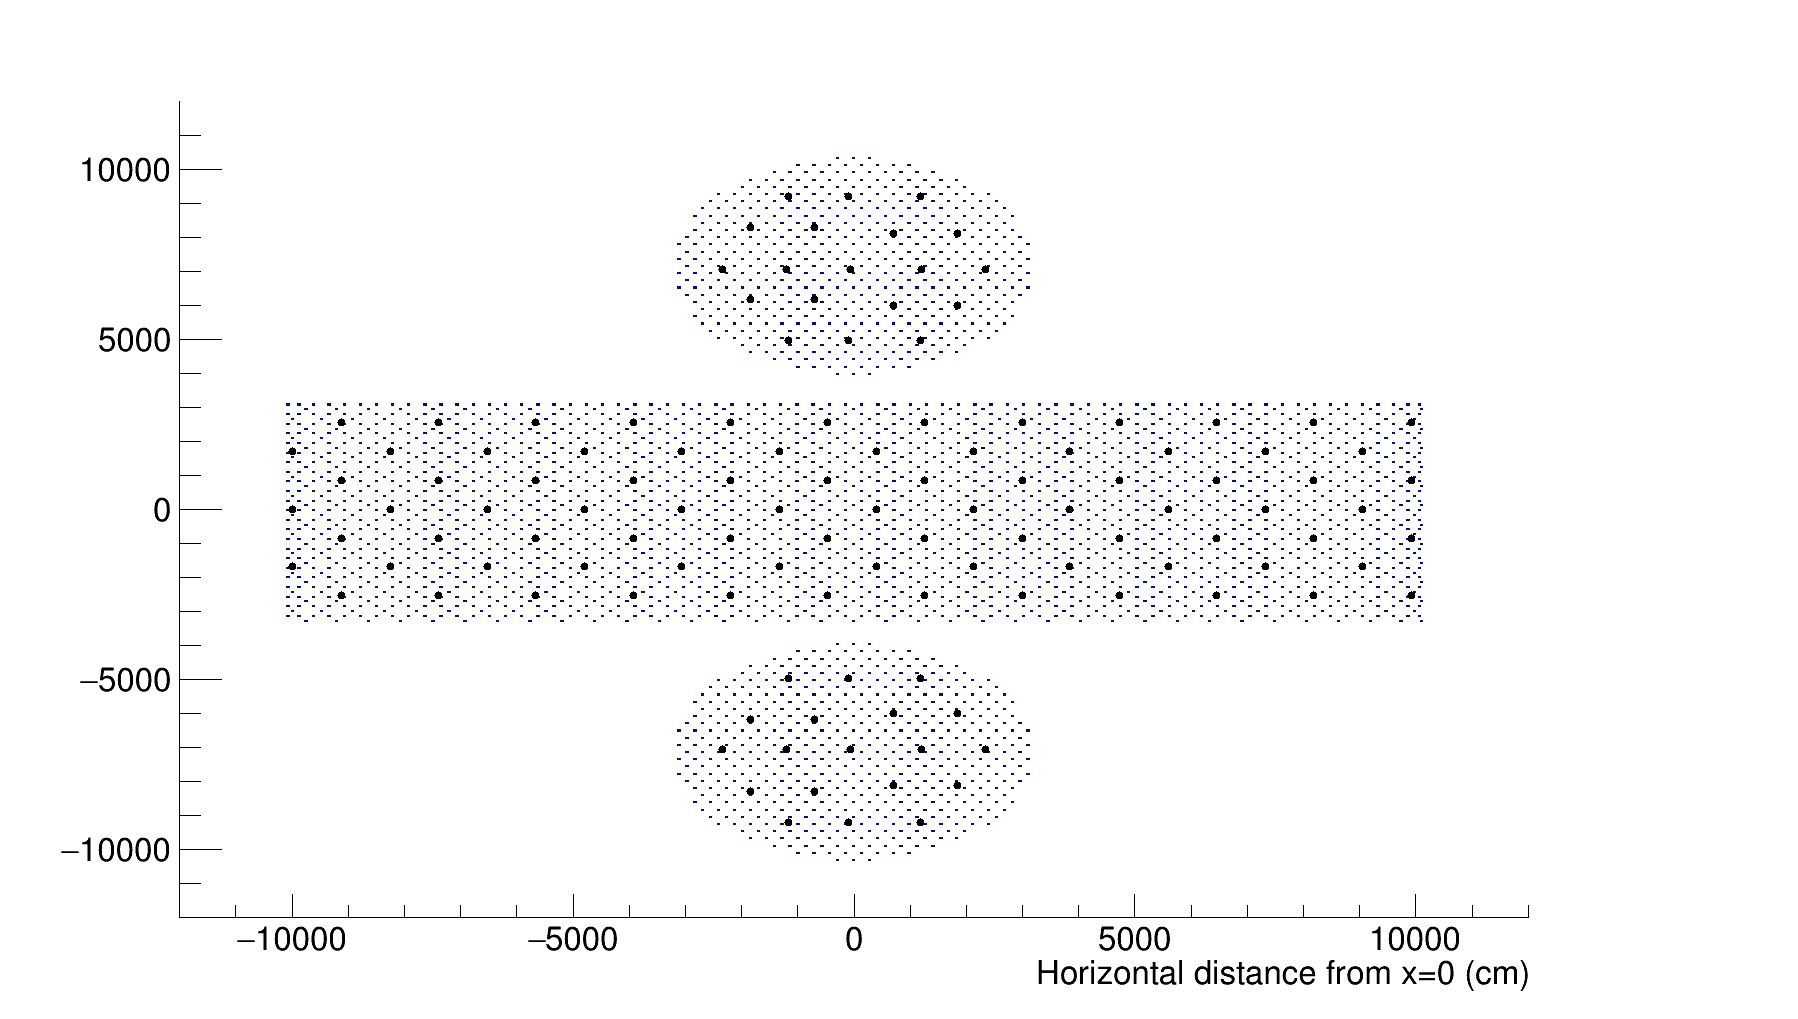
\includegraphics[width=0.95\linewidth]{diffuser_PMT_positions.png}
    \caption{Positions of the OD PMTs and diffuser positions used in the calibration simulations. Note that the positions of PMTs in the top and bottom rows of the barrel have changed in the design, and as such the results presented in this tech note reflect these changes. This differs from the most recent version of WCSim (1.12.26)~\cite{WCSim} that has been used as a basis for the simulation, and the changes are reflected in pull request \#525.}
    \label{fig:diffuserPositions}
\end{figure}

A new LI generator has been written within the framework of WCSim~\cite{WCSim}. This allows the user to define the characteristics of the LI within a data file input to the simulation. The following characteristics can be defined:
\begin{itemize}
    \item Global position within the detector geometry,
    \item Direction of the LI axis,
    \item Wavelength of the optical photons
    \item Pulse width
    \item Photons per pulse
    \item LI profile in the form of arrays of $\theta$, $\phi$ and measured light intensity, where $\theta$ is the angle made with the axis of the LI and $\phi$ is the rotation around the axis.
\end{itemize}

The LI profile opening angle and intensity can reflect either a flat angular distribution of photons within the desired angular range of the light injector (-opening angle, +opening angle), or can be drawn from the measured profile for that injector, in which case the LI generator accurately models the variation across the profile, and in particular the drop-off in the frequency of photons towards the edge of the LI profile. For each pulse, the generator samples the specified number of photons per pulse, each with an energy calculated from the wavelength set in a database currently stored within WCSim, and a time sampled from a Gaussian distribution around the mean, with a variance equal to the pulse width specified in the database. Each photon is also assigned a global direction, which is sampled with a distribution corresponding to the LI profile.

The profile of each diffuser will be measured and stored in the database as a function of the diffuser identifier number in the final simulation. For the purposes of the diffuser simulations presented in this tech note, a single diffuser profile taken from the measurement of a diffuser profile in water has been used. This diffuser profile corresponds to an opening angle of around 40\textdegree. Since the OD diffuser profiles have not yet been measured in water, an ID diffuser profile has been used to approximate a realistic OD diffuser profile. Although the design of the OD diffusers has been modified from the ID diffuser design in order to increase the diffuser efficiency, the design has been shown to maintain the desired profile and as such the ID diffuser profile is expected to be a reasonable approximation. The diffuser profile used, and the resulting charge map from a diffuser in the barrel is shown in \cref{fig:diffuserProfileSim}.

\begin{figure}
    \centering
    \begin{subfigure}{0.45\textwidth}
         \centering
         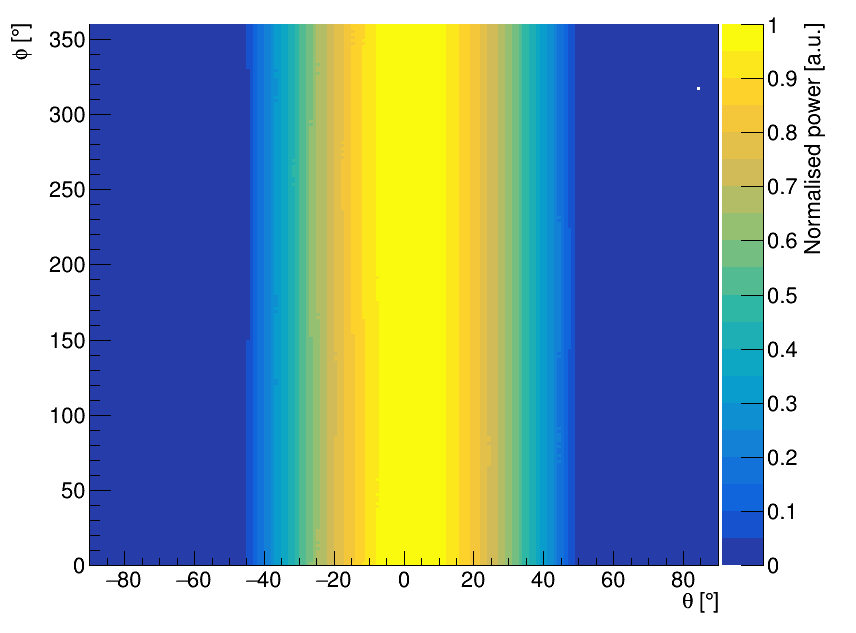
\includegraphics[width=\linewidth]{Differ_profile.png}
         \caption{ID diffuser profile measured in water, used for the diffuser simulations described in this technical report. A measured profile for each diffuser will be stored in the database for OD calibration.}
         \label{fig:diffuserProfile}
     \end{subfigure}
     \hfill
     \begin{subfigure}{0.5\textwidth}
         \centering
         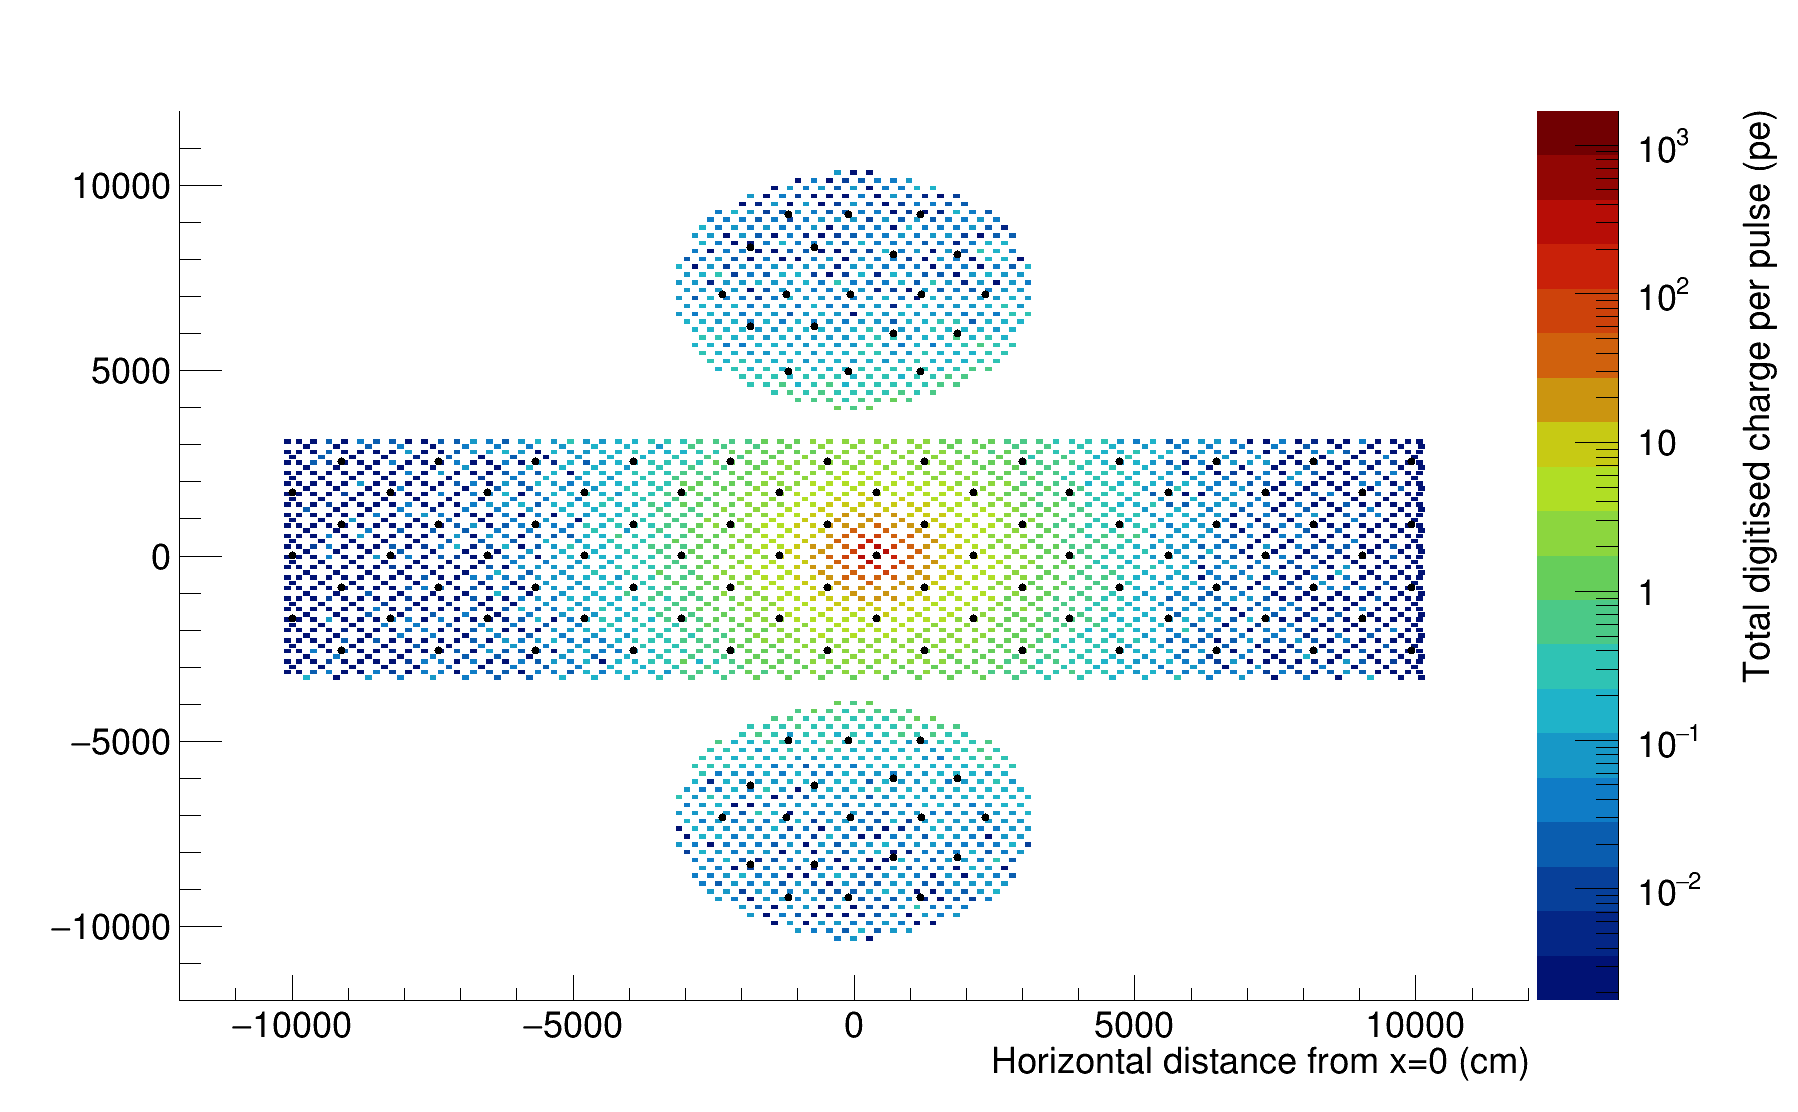
\includegraphics[width=\linewidth,height=5cm]{diffuse_QCoverage.png}
         \caption{Charge in photoelectrons on each PMT produced when the profile in (a) is used to simulate optical photons from a diffuser pointing outwards in the barrel OD. The size of the PMT + WLS plates has been increased only in the plot for improved visualisation.}
         \label{fig:diffuserChargeMap}
     \end{subfigure}
     \caption{Diffuser profile measured in water, and the resulting charge map from this profile.}
     \label{fig:diffuserProfileSim}
\end{figure}

\subsection{Diffuser and OD Parameters}\label{subsec:params}

The characteristics of diffusers simulated in the Saturation Study are summarised in \cref{tab:satStudyParams}. The number of photons per pulse used in the simulation was modified to account for optical photon attenuation in 100~m of optical fibre and a measured diffuser efficiency of 50\%. As such, the simulated number of photons per pulse is 5.5~M.

\begin{table}[h!]
    \centering
    \begin{tabular}{|c|c|}
    \hline
        Parameter    & Assumed value \\
        \hline
       Photons per pulse  &  23 M\\
       Wavelength  & 365 nm \\
       Pulse width & 10~ns\\
       Attenuation in 100 m of fibre & 50\%\\
       Diffuser efficiency & 50\%\\
       \hline
    \end{tabular}
    \caption{The LI configuration used in the diffuser simulations for the saturation study presented in \cref{subsec:satStudy}.}
    \label{tab:satStudyParams}
\end{table}

The OD geometry parameters that have been used in the simulations for the saturation study are shown in \cref{tab:od_config}.

\begin{table}[h!]
    \centering
    \begin{tabular}{|c|c|}
    \hline
        Parameter    & Assumed value \\
        \hline
       PMT radius  &  8~cm\\
       PMT dark rate & 0.4 kHz \\
       OD lateral water depth  & 1 m \\
       OD height water depth & 2 m\\
       OD dead space & 60 cm \\
       Tyvek sheet thickness & 1 mm\\
       WLS plate thickness & 6 mm \\
       WLS plate length & 30 cm \\
       \hline
    \end{tabular}
    \caption{The OD configuration used for the saturation study presented in \cref{subsec:satStudy} using WCSim version 1.12.26.}
    \label{tab:od_config}
\end{table}



\subsection{Saturation Study}\label{subsec:satStudy}

The limit of the PMT range is governed by the electronics response, which is expected to fully saturate at around 100 photoelectrons (pe) in a 16~ns time window. The simulation of the PMT charge response in WCSim does not currently handle the saturation, but it is expected that the linearity of the charge response will break down between 80~pe and 100~pe. Saturation measurements aim to measure the PMTs over the full range of this breakdown in linearity. The saturation level for the purposes of this study has been taken to be 100~pe in 16~ns, but the analysis has been designed to take into account the need to measure across the entirety of this range.

The saturation of OD PMTs has been evaluated in the top endcap, barrel and bottom endcap. The diffuser simulations are intensive, requiring millions of tracked photons to simulate a single flash. As such, only two diffusers in each of the top endcap, barrel and bottom endcap have been simulated for this current study.

Two values have been used as figures of merit to determine the PMT saturation coverage:
\begin{itemize}
    \item Mean saturation distance - the distance from the nearest diffuser at which the mean charge per PMT is greater than saturation level.
    \item Saturation limit - the greatest distance from the nearest diffuser at which the charge on any PMT reaches the saturation level.
\end{itemize}

For each configuration, the charge per PMT was plotted as a function of the distance from the nearest diffuser, to give the saturation limit (\cref{fig:maxSatDistPlot}). The mean saturation distance was then found by taking the mean of the same plot (\cref{fig:meanSatDistPlot}). The plot showing the saturation limit is particularly useful in understanding the range of distances over which it is possible to see the expected range of breakdown of linearity.

\begin{figure}[h!]
    \centering
    \begin{subfigure}{0.49\textwidth}
         \centering
         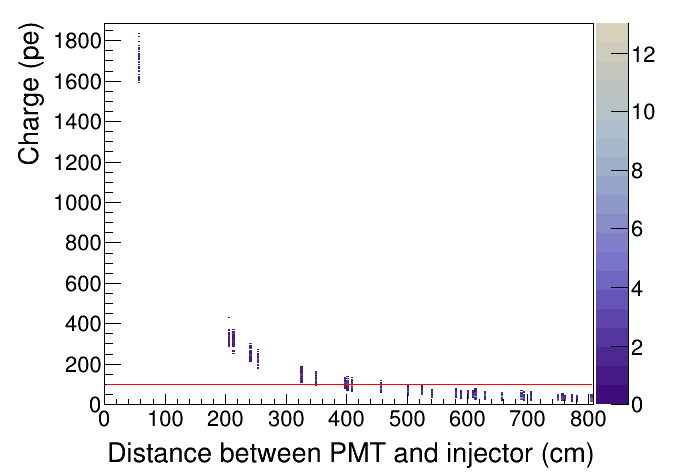
\includegraphics[width=\linewidth, height=5.2cm]{charge_distance_reduced_diffuser_41_365.0_nm_10.0_ns_5500000_ppp_all.png}
         \caption{Plot of the charge per PMT as a function of the distance from the nearest diffuser. The saturation limit is the greatest distance at which saturation is achieved i.e. 5.0~m in this case.}
         \label{fig:maxSatDistPlot}
     \end{subfigure}
     \hfill
     \begin{subfigure}{0.49\textwidth}
         \centering
         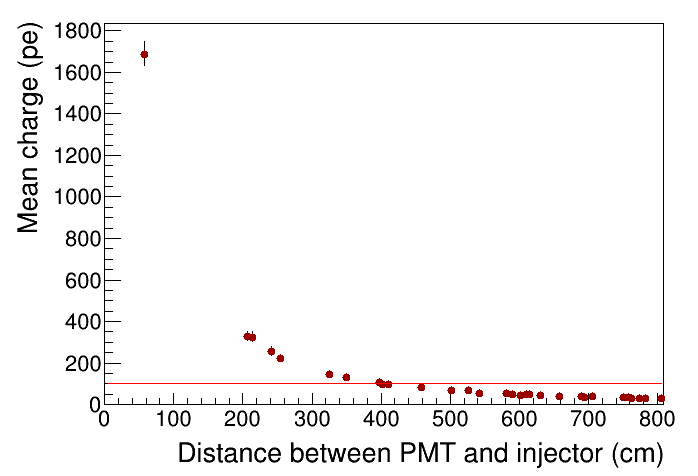
\includegraphics[width=\linewidth,height=5cm]{mean_charge_distance_reduced_diffuser_41_365.0_nm_10.0_ns_5500000_ppp_all.png}
         \caption{Plot of the mean charge per PMT found by taking the mean of the left-hand plot. The mean saturation distance is the greatest distance at which the mean charge per PMT is greater than the saturation level i.e. 4.0~m.}
         \label{fig:meanSatDistPlot}
     \end{subfigure}
     \caption{Sample plots showing the mean saturation distance and saturation limit used as figures of merit for the saturation study. The red, horizontal lines mark the assumed saturation level of 100~pe.}
     \label{fig:satAnalysisPlots}
\end{figure}

Since only six diffuser locations have been simulated, the percentage of PMTs within the mean saturation distance and saturation limit is calculated assuming symmetry both of the detector and of the diffuser positions with respect to the PMTs. However, for practical reasons, the diffusers have to be positioned off-centre in the empty cells between PMTs, next to the struts on the PMT support structure. As such, a full simulation of all diffusers should be performed in future, once the OD geometry and LI specifications have been finalised, for an accurate evaluation of the percentage saturation across the whole detector.

\subsection{Results}\label{subsec:results}

The mean saturation distance and saturation limit were evaluated for two OD diffuser locations in each of the top endcap, barrel and bottom endcap. These are shown in \cref{tab:satStudyResults}, along with the percentage of PMTs within the mean saturation distance and saturation limit. \cref{tab:satStudyResults_pevalues} shows the mean charge at the calculated saturation distance and the mean charge at the saturation limit at the six diffuser positions.
\begin{table}[h!]
    \centering
    \begin{tabular}{|c|c|c|c|c|}
    \hline
        OD location & Mean saturation & \% PMTS within & Saturation  & \% PMTs within \\
                    &  distance & saturation distance & limit &  saturation limit\\
        \hline
        Barrel 1        & 4.0~m & 31\%        & 5.0~m   & 50\% \\
        Barrel 2        & 4.0~m    & 31\%     & 5.0~m   & 50\% \\
		Top endcap 1    & 3.7~m  & 27\%       & 3.9~m & 30\% \\
        Top endcap 2    & 3.6~m  & 24\%       & 4.3~m & 37\% \\ 
		Bottom endcap 1 & 3.6~m  & 24\%       & 4.3~m & 37\% \\
		Bottom endcap 2 & 3.5~m  & 22\%       & 6.1~m & 66\% \\
        \hline
    \end{tabular}
    \caption{Results for PMT saturation using the diffuser configuration detailed in \cref{tab:satStudyParams}.}
    \label{tab:satStudyResults}
\end{table}
%
\begin{table}[h!]
    \centering
    \begin{tabular}{|c|c|c|c|}
    \hline
        OD location &Diffuser position & Mean charge (pe) at  & Mean charge (pe) at   \\
                    &                  & saturation distance & saturation limit $\pm2\sigma$.  \\
        \hline
        Barrel 1       & (395.65,-3281.50,8.75 cm)   & 108  & 68 $\pm$ 12 \\ 
        Barrel 2       & (3281.50,395.65,1705.55 cm) & 105  & 67 $\pm$ 11 \\ 
        Top endcap 1   & (-70.7,-97.3,3350.82 cm)    & 106  & 96 $\pm$ 14 \\
        Top endcap 2   & (-707,-968.2,3350.82 cm)    & 108  & 77 $\pm$ 13 \\
        Bottom endcap 1 & (-707,-968.2,-3350.82 cm)  & 108  & 77 $\pm$ 14 \\ 
        Bottom endcap 2 & (707,-1157.8,-3350.82 cm)  & 114  & 42 $\pm$ 11 \\ 
        \hline
    \end{tabular}
    \caption{Results for PMT saturation using the diffuser configuration detailed in \cref{tab:satStudyParams}.}
    \label{tab:satStudyResults_pevalues}
\end{table}

\cref{fig:pmtmap_with_limits} shows the PMT charge map for the Barrel 1 diffuser, with the saturation distance and saturation limits marked around the barrel PMTs.

\begin{figure}
\centering
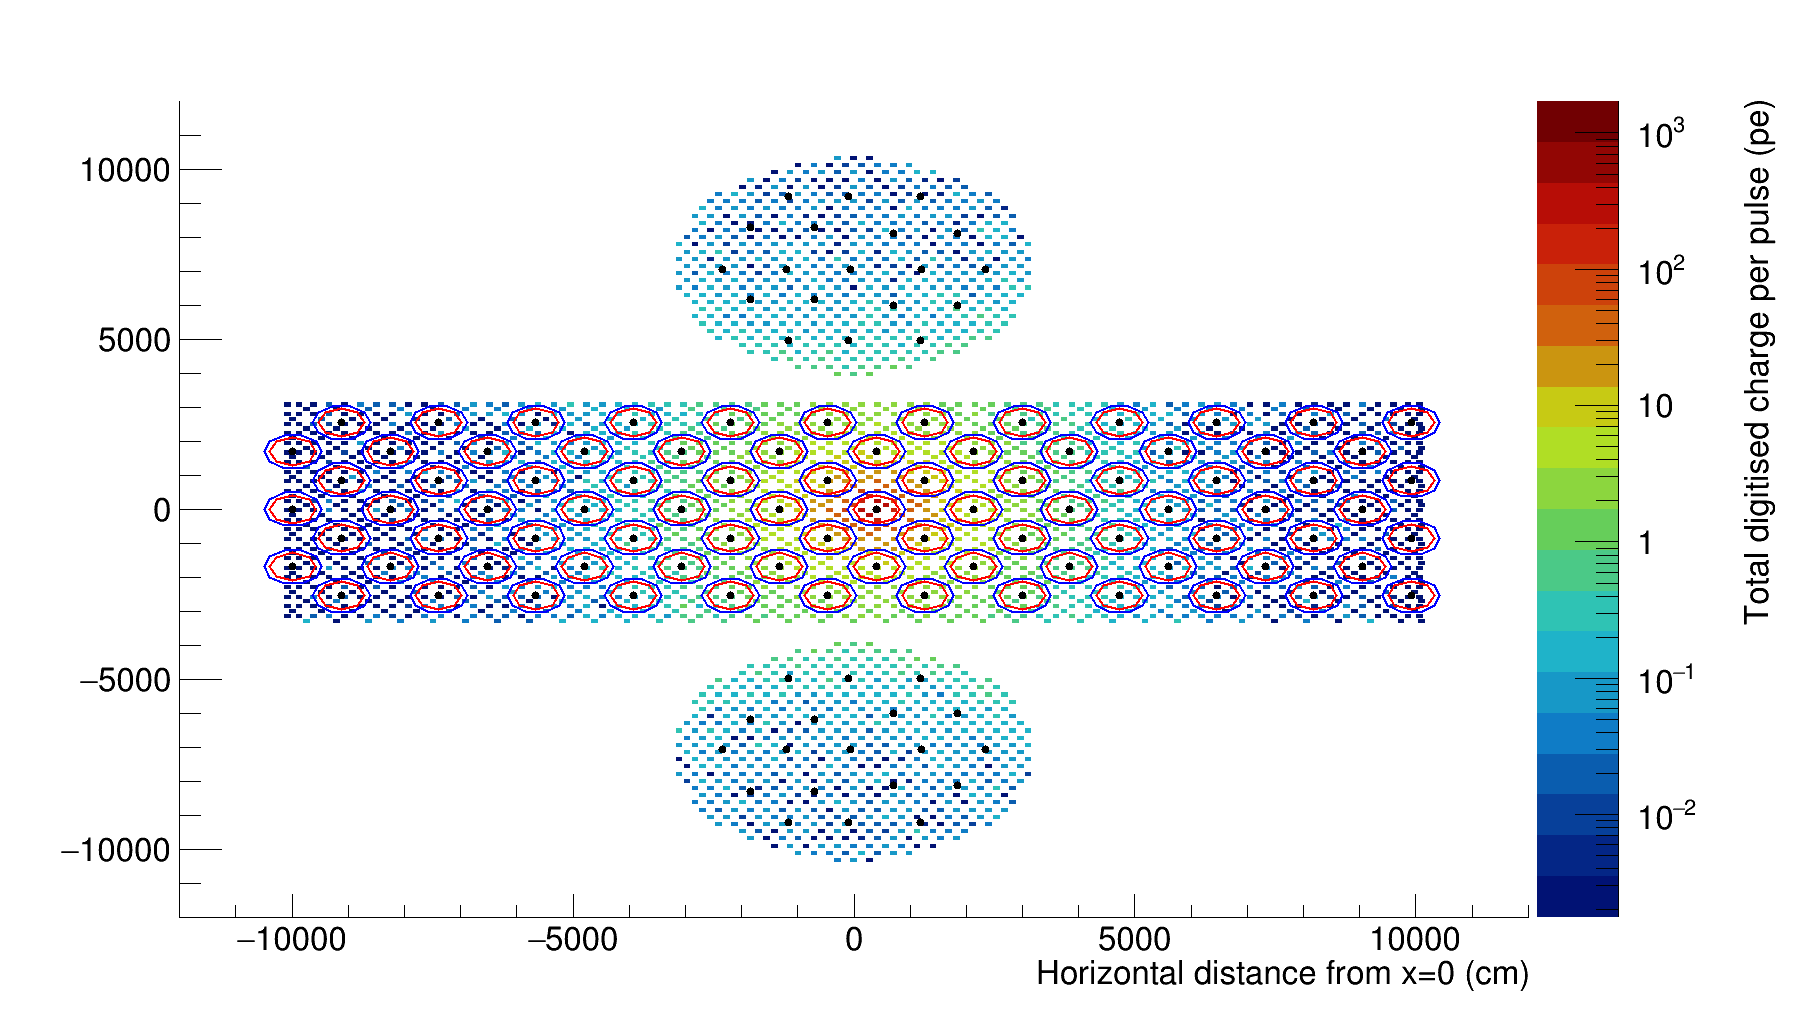
\includegraphics[width=0.7\linewidth]{diffuse_QCoverage_with_limits.png}
         \caption{Charge in pe on each PMT as a result of illumination with the Barrel 1 diffuser. The mean saturation distance and saturation limit around each PMT in the barrel are marked in red (smaller circles) and blue (larger circles) respectively.}
         \label{fig:pmtmap_with_limits}
\end{figure}

Due to the differing geometry the mean saturation distance in the barrel (4.0~m) is slightly higher than in the endcaps (e.g. 3.6~m), and the percentage of PMTs within the mean saturation distance in the barrel is higher at 31\% than in the endcaps (22-27\%). Similarly, the percentage of PMTs within the saturation limit in the barrel is higher than in the endcaps, with the exception of the bottom endcap 2 diffuser, with 66\% of PMTs within the saturation limit of 6.1~m. It should be noted that changes to the OD geometry, including the addition of PMTs in the endcaps, are possible, and have not been taken into account in this simulation. 

The diffuser position with respect to the surrounding PMTs has an observable effect on the saturation levels achieved. Where the diffuser positions with respect to surrounding PMTs are equivalent, as in the case of the two barrel diffusers, as well as the Bottom Endcap 1 and Top Endcap 2 diffusers, saturation levels are largely the same. However, the positions of the Top Endcap 1 and Bottom Endcap 2 diffuser each differ from all other diffusers simulated, resulting in different saturation distances and saturation limits.   Again, a full simulation of all diffuser positions should be carried out to fully evaluate achievable saturation across the whole detector, once all parameters and geometries have been finalised.

\section{Diffuser Design}\label{sec:diffuser}
\subsection{ID Diffuser Hemisphere Design}
\subsubsection{Inner Detector Diffuser Design}

The diffusers used to scatter input laser light in the inner detector volume are 2.54~cm half-spheres fabricated from PTFE. This is used as it
\begin{itemize}
\item is unaffected by immersion in water
\item acts as a excellent diffuser
\item is a good transmitter of UV light
\item is easy to machine and clean
\end{itemize}

A mechanical drawing of the inner detector diffuser hemispheres is shown in \cref{fig:Bare_Diffuser_Mechanical}

\begin{sidewaysfigure}
    \centering
    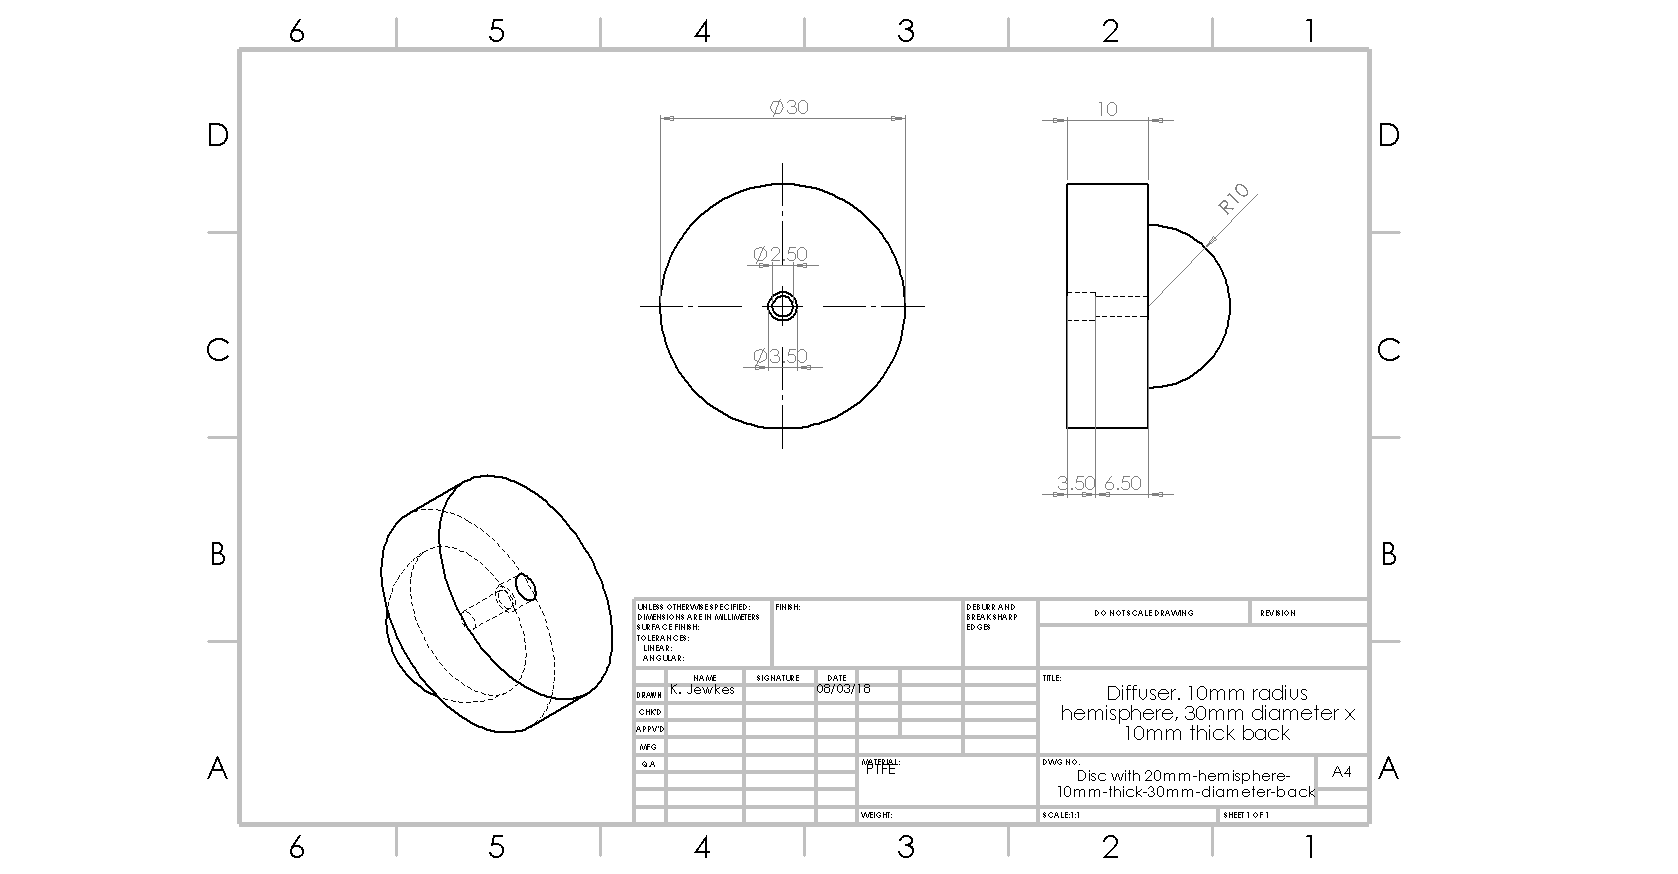
\includegraphics[width=\textwidth]{BareDiffuser.PNG}
    \caption{Bare Diffuser Mechanical Drawing}
    \label{fig:Bare_Diffuser_Mechanical}
\end{sidewaysfigure}

\subsubsection{Diffuser Profile Measurement System}

\begin{figure}[t]
    \centering
    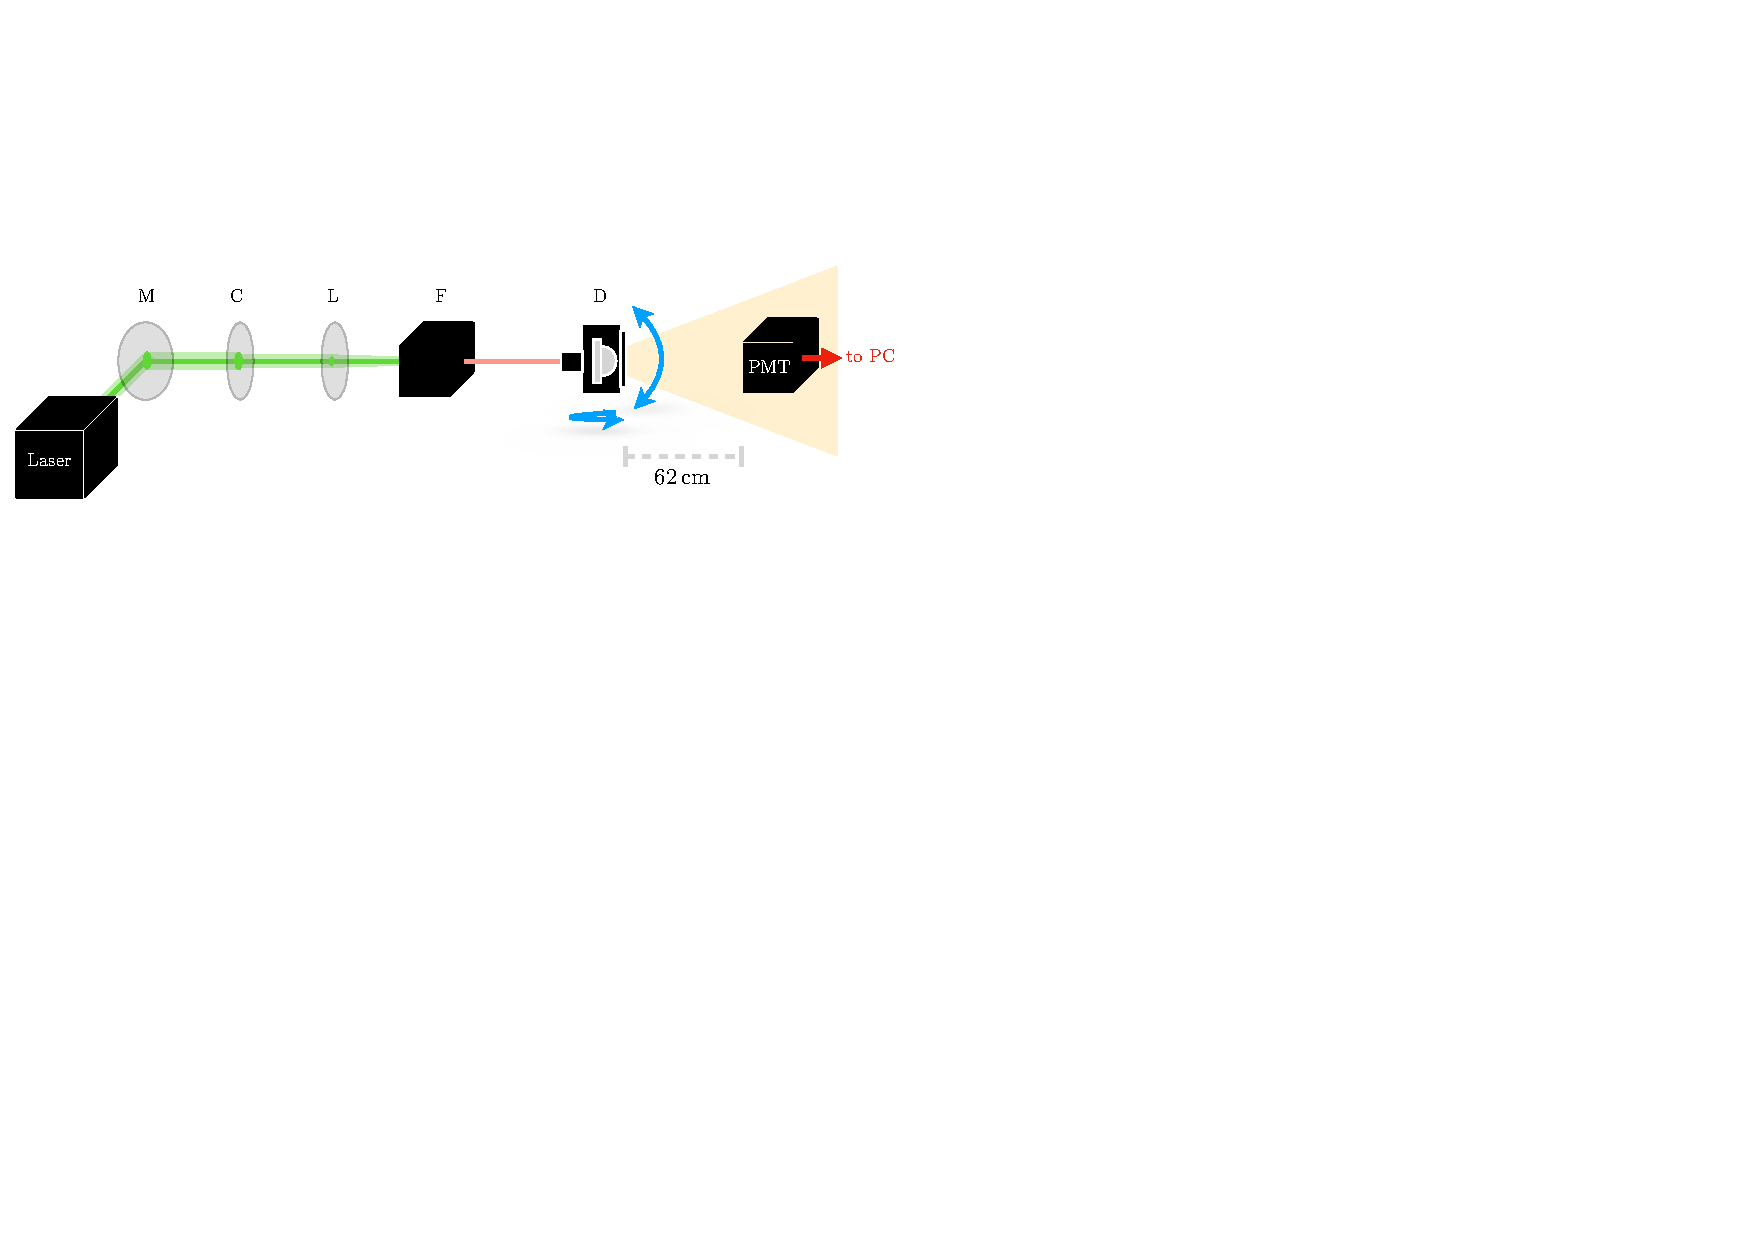
\includegraphics[width=\textwidth]{diffuser_setup_new.pdf}
    \caption{Setup for diffuser scans: light from the laser is directed via a mirror (M), a circulator (C), and a lens (L) to the fibre launch stage (F). From there, the light goes via an optical fibre to the diffuser (D) on the rotation stage.}
    \label{fig:setup}
\end{figure}

A scanning system was built to measure the output characteristics of diffuser hemispheres. Enclosed in a dark box, the diffuser is mounted onto two rotary stages which gives the freedom to rotate the diffuser around the nominal axis linking the diffuser with the photosensor. This scanner only takes scans in an air medium, and the setup is illustrated in \cref{fig:setup}. 

A laser powered from a wall plug is used to illuminate the diffuser with light at  a wavelength of 450~nm. It is triggered by a function generator with 1000 triggers per burst at a frequency of 2~kHz. 
The open beam is directed via a mirror, a circulator, and a lens to the fibre launch stage, and then via an optical fibre towards the diffuser. The diffuser enclosure is fixed with three screws on the double-rotation stage. Measurements of bare diffuser profiles, i.e. without enclosure, are conducted with the bare fibre end positioned in the centre of the rotation stage using a 3D printed frame. The bare fibre end is kept in place due to friction on the connection point with the diffuser hemisphere. A photograph of the rotation stage with a bare diffuser hemisphere is  shown in \cref{fig:difftest_rotstage}.

\begin{figure}
    \centering    
    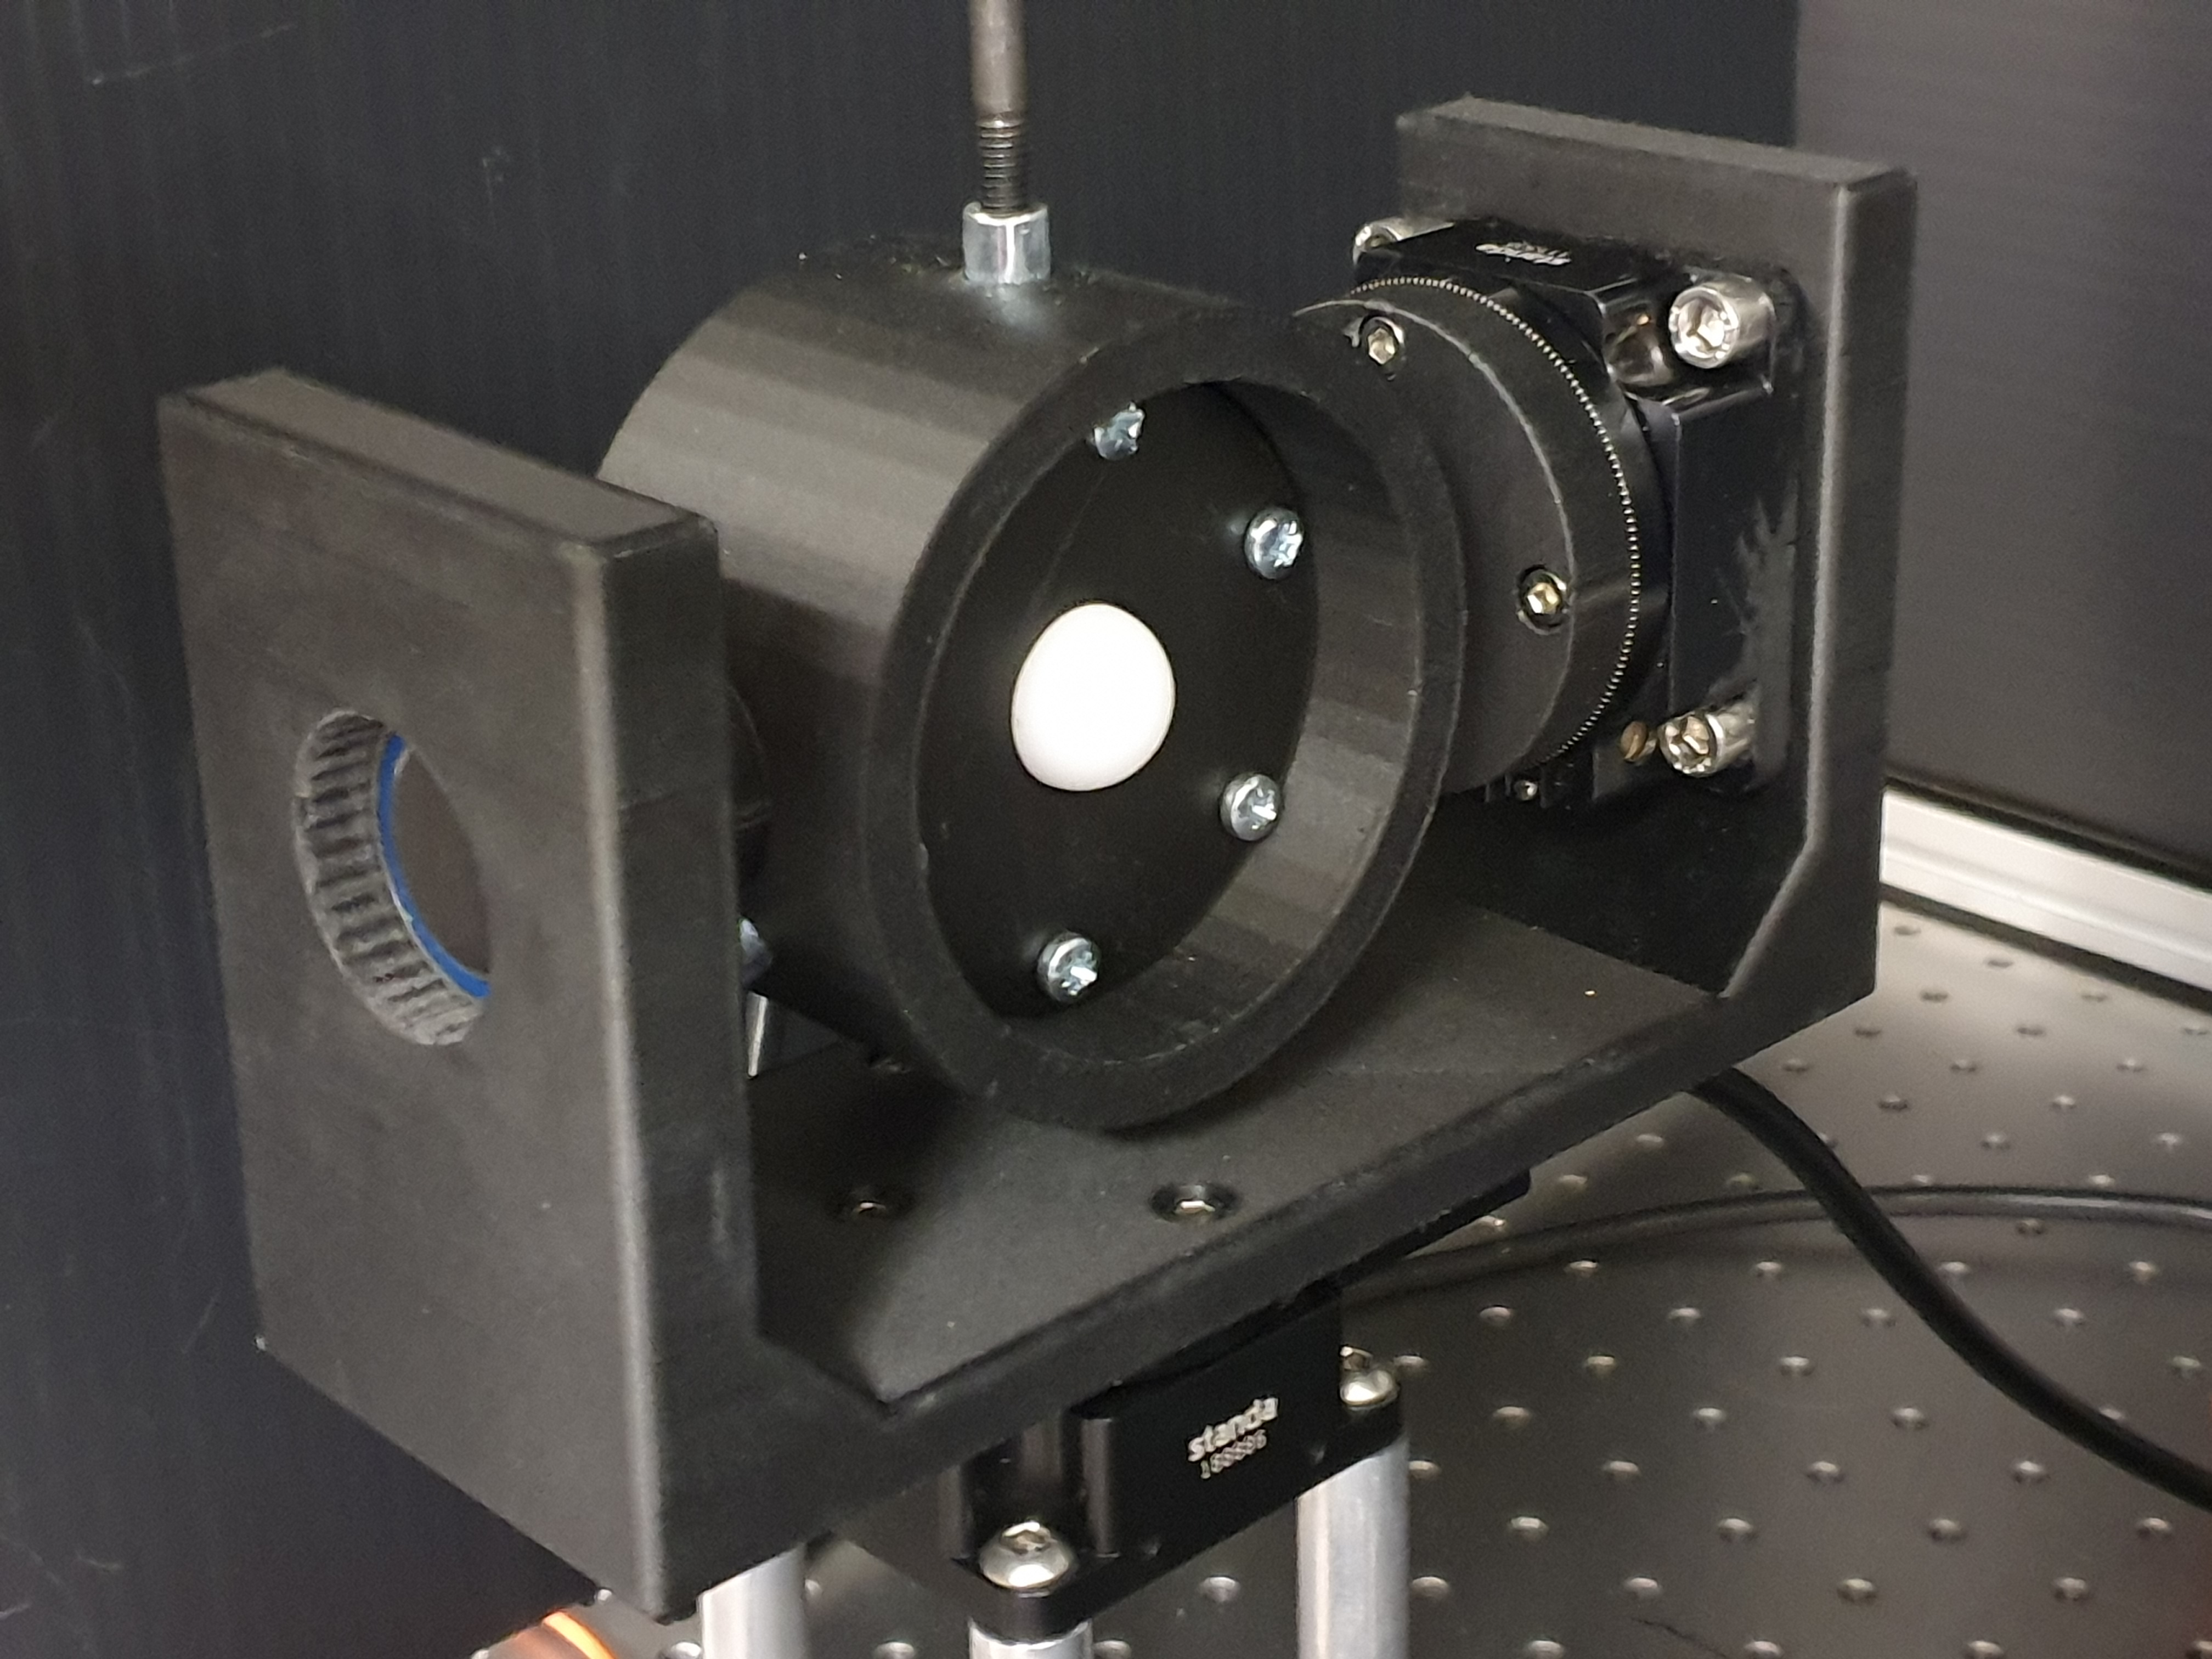
\includegraphics[height=.35\textwidth]{bare_scan_setup.jpg}%
    \caption{Rotation stage with bare diffuser hemisphere mounted using a 3D-printed frame.} 
    \label{fig:difftest_rotstage}
\end{figure}

A PMT measures the diffuser spectrum at a fixed position, with 62~cm distance to the diffuser enclosure and a 3~mm pinhole aperture, restricting the solid angle viewed by the PMT to $2\cdot10^{-5}$~sr. For comparison, a single 50~cm PMT in the HK far detector receives light from a point source at the other side of the tank over a solid angle of approximately $2.2\cdot10^{-4}$~sr.
The PMT signal is digitised at a sampling rate of 2500~MHz over 1000 cycles, allowing to resolve the shape of each single signal waveform. The light yield at each coordinate is then obtained as the average waveform area across all digitised signals. 

\begin{figure}[h]
  \centering
  \begin{subfigure}[b]{0.45\textwidth}
    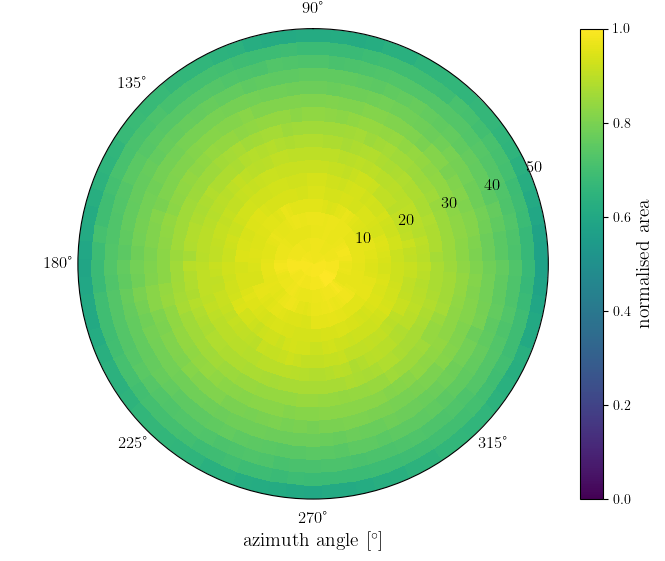
\includegraphics[width=\linewidth]{b71_polar.png}
    \caption{2D polar histogram of bare ID hemisphere}
    \label{fig:bare polar}
  \end{subfigure}
  \hfill
  \begin{subfigure}[b]{0.45\textwidth}
    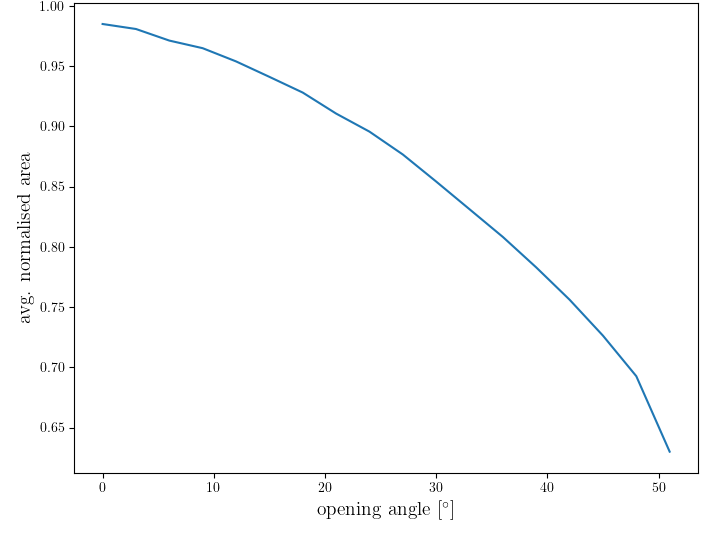
\includegraphics[width=\linewidth]{b71_radial.png}
    \caption{Radial profile of bare ID hemisphere}
    \label{fig:bare radial}
  \end{subfigure}
  \caption{Profile scan of a standard bare ID diffuser hemisphere}
  \label{fig:bare scan}
\end{figure}

The diffuser profile measurement system is discussed in detail in \cite{TN42}.

\subsubsection{Diffuser Power Measurement System}

In addition to the profile measurement functionality, the integrated power output from the diffuser was measured using an integrating sphere from Ophir. This sphere provides an unbiased measurement of the total light output power of any light source, regardless of the shape of the emission profile. A bespoke diffuser holder suitable for connection to one of the integrating sphere ports was 3D-printed, as was a holder for the optical fibre from the laser source. 

A bare PTFE hemisphere was mounted into this holder and connected into the integrating sphere port. The bare end is inserted into the connection point in the same manner as for a bare profile scan. Tape was used to in order to prevent light leaking out of the back of the hemisphere during the measurement, which also helped to keep the fibre in place. The hemisphere was then illuminated with light from the same laser, this time running on a continuous rather than burst setting. On the continuous setting light is supplied in a sinusoidal manner at a frequency of 1~kHz. Power measurements were taken once per second for a period of ten seconds to account for small fluctuations in laser intensity, the mean of which served as the final power measurement for that hemisphere. 

In order to calculate a power ratio, a measurement of power for the bare fibre also needed to be obtained. This was done in a similar manner to a power measurement for a hemisphere, using the same laser and data acquisition settings. To make the comparison between fibre and hemisphere measurement as accurate as possible, a special hemisphere was created with the fibre connection point extended into a hole that runs through the length of the hemisphere. The bare fibre can then be inserted all the way through until it pokes out of the front, allowing a power measurement for the bare fibre to be taken with the conditions inside the integrating sphere as close as possible to hemisphere measurements. The ratio of hemisphere power to fibre power can then be taken to determine the amount of light lost.


A table of systematics for the power ratio measurement is shown in \cref{tab:systematics}. Rotation refers to changing the orientation at which the diffuser is placed into the holder, and diffuser re-insertion refers to removing the diffuser from the holder and replacing it. Fibre re-insertions refers to disconnecting and re-connecting the fibre into the diffuser, while bare fibre refers to dis- and re-connecting the fibre when taking bare fibre measurements. This results in a total systematic of $5.3\%$ for a diffuser measurement and $1.8\%$ for a fibre measurement, and therefore an uncertainty of $5.6\%$ in a power ratio measurement.

\begin{table}[h!]
\centering
\begin{tabular}{|c|c|}
\hline
Systematic & Std. dev. (\%) \\
\hline
Rotation & 1.4  \\
Diffuser re-insertion & 1.0 \\
Fibre re-insertion & 5.0 \\
Bare fibre re-insertion & 1.8 \\
\hline
\end{tabular}
\caption{Integrating sphere systematics for the power ratio measurement.}
\label{tab:systematics}
\end{table}

\subsection{OD Diffuser Design}

The original intention was to use the same diffuser hemisphere design for the OD diffusers as will be used for the ID diffusers.  However, the standard diffuser emits less than 20\% of the power delivered by an optical fibre. As there are a number of interfaces in the optical pathway between the light source and the diffuser, and as the light source for the OD will be LEDs, this was considered too low to be able to effectively illuminate the OD space. Neither the number of interfaces in the optical chain, nor the light source can be changed easily, but it is possible that an alternate design of the diffuser hemisphere could yield more light.

\begin{figure}
    \centering    
    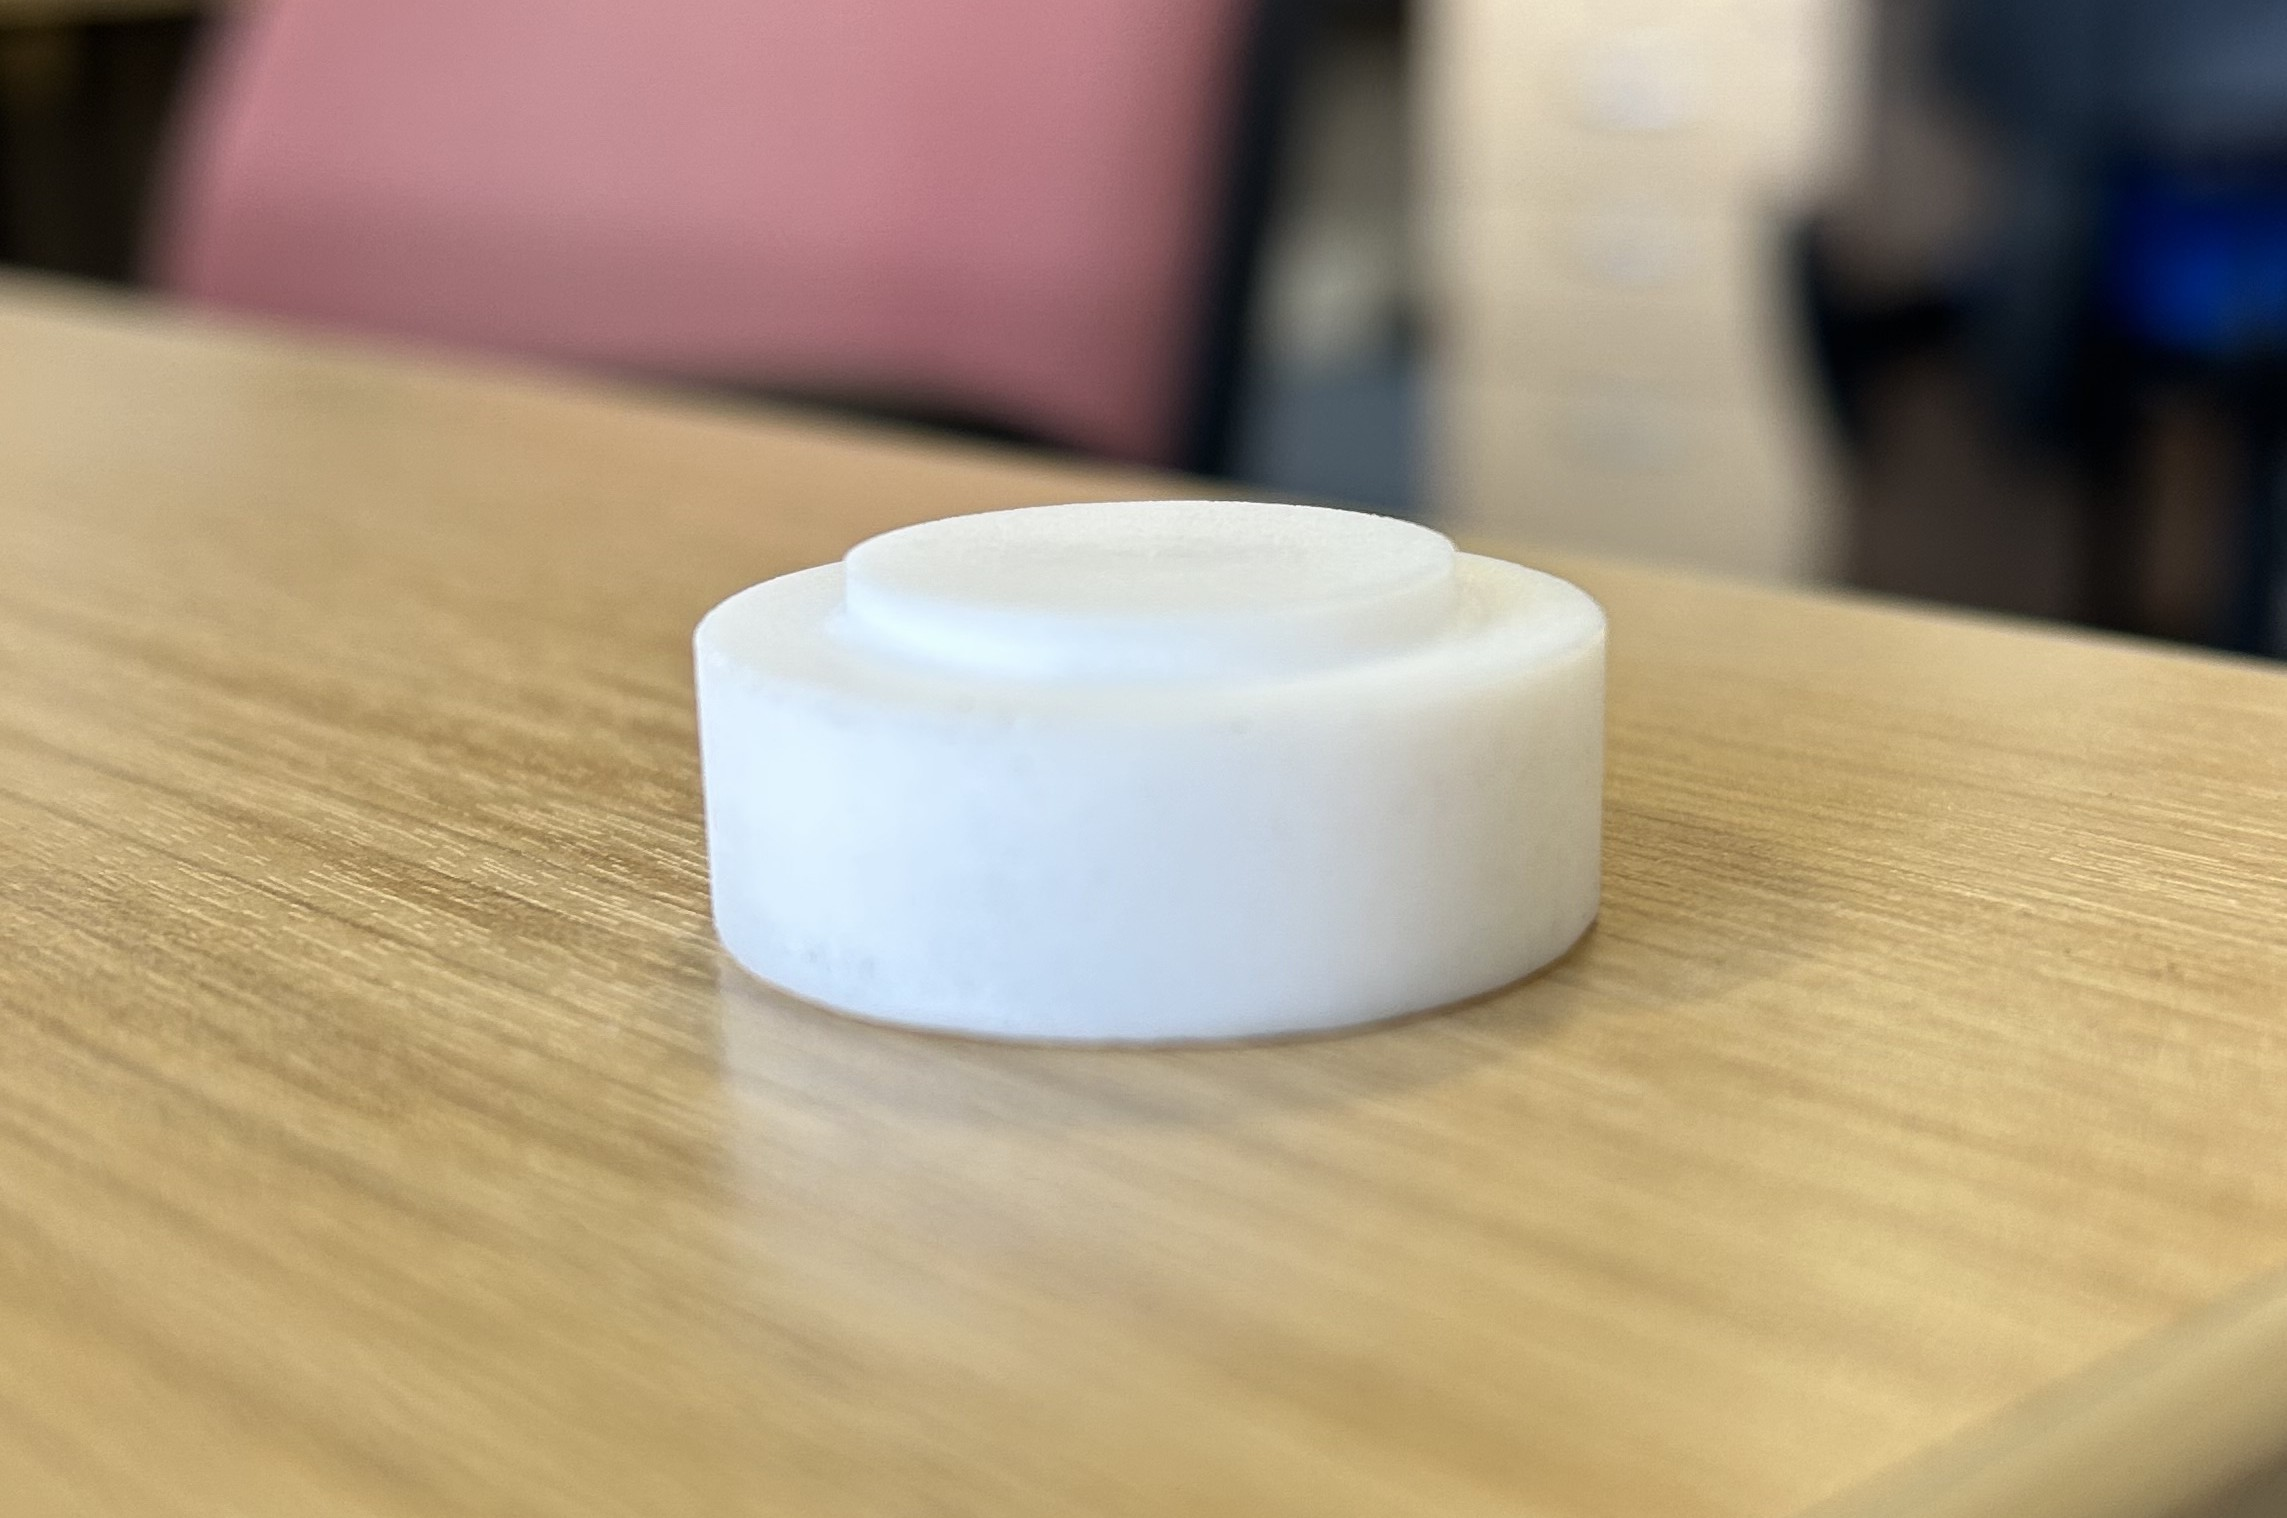
\includegraphics[height=.35\textwidth]{2mm_tophat_side.jpg}%
    \caption{A prototype of the OD diffuser with a 2~mm top hat.} 
    \label{fig:topHat}
\end{figure}

Light is lost to two mechanisms in the standard diffuser; absorption by the PTFE and backscattering. Both loss mechanisms would be minimised if there were less PTFE in the light path. The design for the OD diffuser section was modified to be the shape of a top hat, as shown in \cref{fig:topHat}. The optimal depth was studied by taking profile and power ratio measurements using the same diffuser, but at smaller and smaller depths; after each measurement was completed, 2.0~mm was cut from the top-hat, and the measurements were re-taken. This procedure was repeated until the top-hat was 2.0~mm high.

\begin{table}[h!]
\centering
\begin{tabular}{|c|c|}
\hline
Top-hat depth (mm) & Power ratio (\%) \\
\hline
10.0 & 19.2  \\
8.0 & 32.4 \\
6.0 & 31.5\\
4.0 & 42.1 \\
2.0 & 55.2 \\
\hline
\end{tabular}
\caption{Power ratio measurements for each depth of the top-hat}
\label{tab:top hat efficiencies}
\end{table}

Results of the power ratio measurements are shown in \cref{tab:top hat efficiencies}. As expected, power ratio increases with decreasing top-hat depth, making the optimum depth 2.0~mm. The profile as shown in \cref{fig:2mm top hat profile} confirms that the shape of the profile is still suitable.

\begin{figure}[h]
  \centering
  \begin{subfigure}[b]{0.45\textwidth}
    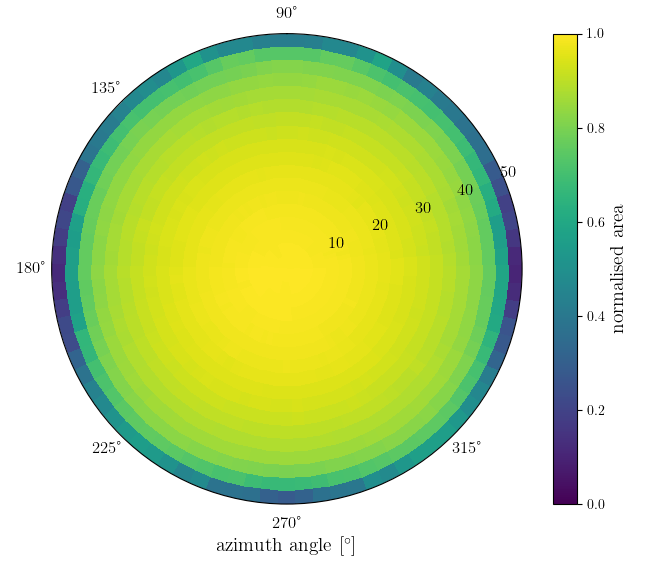
\includegraphics[width=\linewidth]{2mm_tophat_profile.png}
    \caption{2D polar histogram of 2.0~mm top-hat}
    \label{fig:2mm top hat profile polar}
  \end{subfigure}
  \hfill
  \begin{subfigure}[b]{0.45\textwidth}
    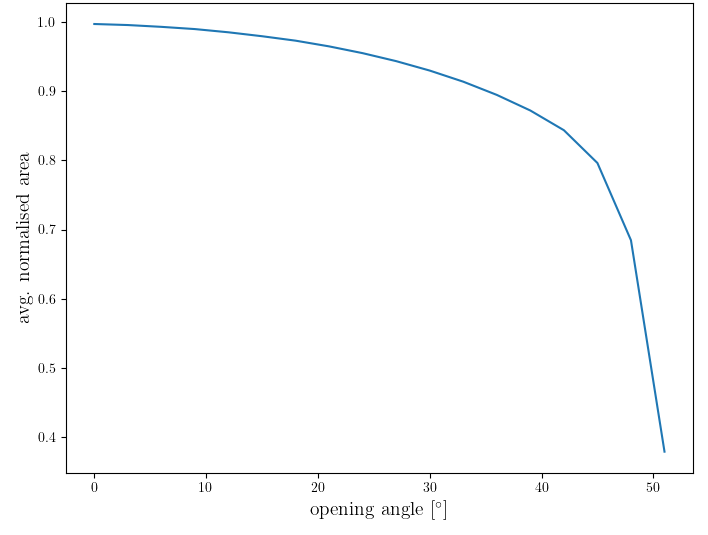
\includegraphics[width=\linewidth]{2mm_tophat_radial.png}
    \caption{Normalised average waveform area vs opening angle for the 2.0~mm top-hat.}
    \label{fig:2mm top hat radial}
  \end{subfigure}
  \caption{Profile scan of the 2.0~mm top-hat}
  \label{fig:2mm top hat profile}
\end{figure}

Based on these studies, we propose to change the OD diffuser design from a hemisphere to a top-hat with a 2.0 mm height above the base. The diffuser will still be fabricated from PTFE, but this new design (i) emits more light at higher emission angles (ii) doubles the amount of light that is emitted for a given LED power setting and (iii) is significantly easier to fabricate in bulk.

\section{OD Diffuser Mounting System and Installation}

The OD space will be illuminated by a total of 122 OD diffusers, 19 on each of the top and bottom caps, and 84 in the barrel. The barrel diffusers are distributed in 7 vertical layers each consisting of 12 OD diffusers. Due to the numbers and cost, the mounting system must be relatively small, easy to fabricate and easy to install. Installation will be carried out by workers on the gondola in the OD space after the Tyvek has been installed and as the fibres are being installed. The gondola worker will install the fibre in the OD diffuser, and fix the mount to the HK frame, oriented into the OD space. Since this is being done on the gondola, the mount needs to be small, easy to store, and straightforward to install.

\begin{figure*}
\centering 
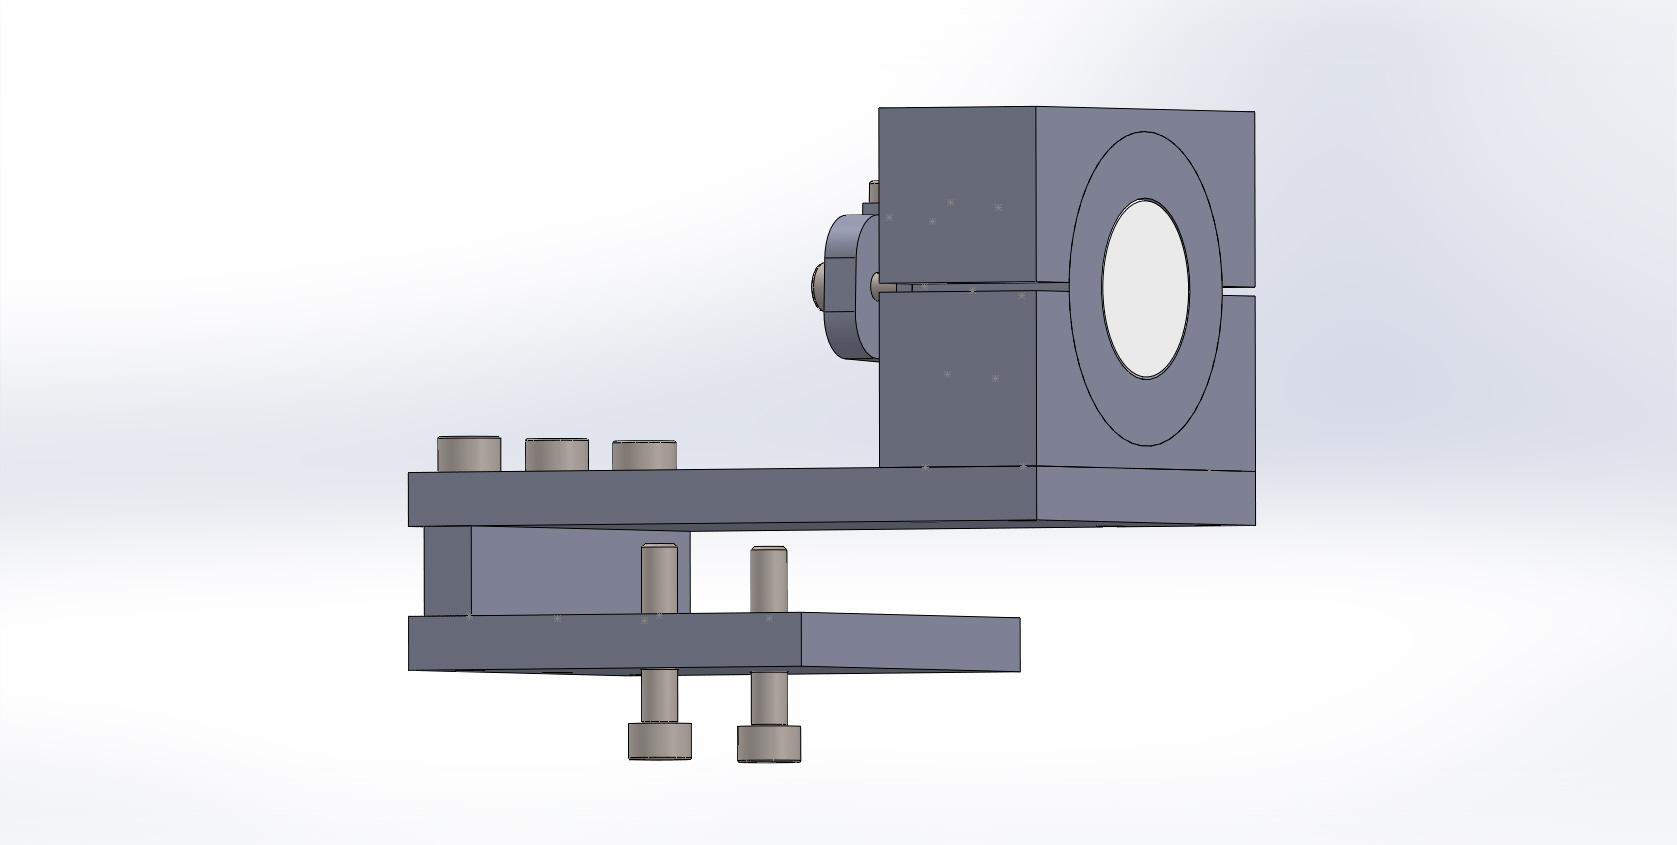
\includegraphics[width=.49\textwidth]{Diffuser-and-mount-complete-top-hat.JPG}%
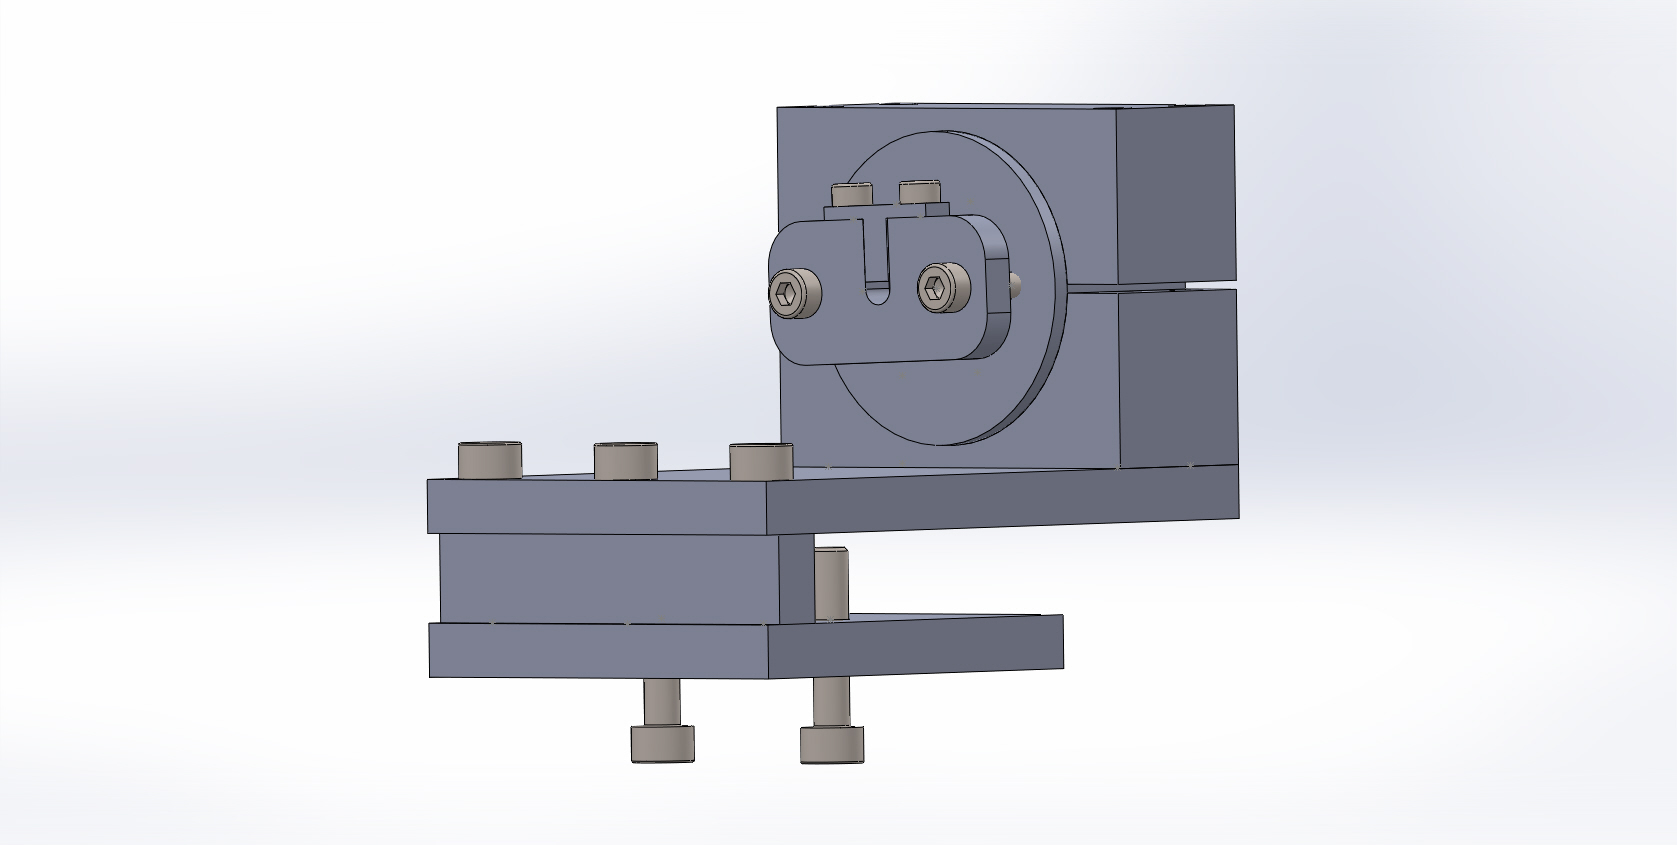
\includegraphics[width=.49\textwidth]{Diffuser-and-mount-complete-top-hat2.JPG}
\caption{(left) Front view of the prototype of the OD diffuser mount and (right) rear view of the prototype of the OD diffuser mount.}
\label{fig:od_diffuser_mount}
\end{figure*}

\begin{figure*}
\centering 
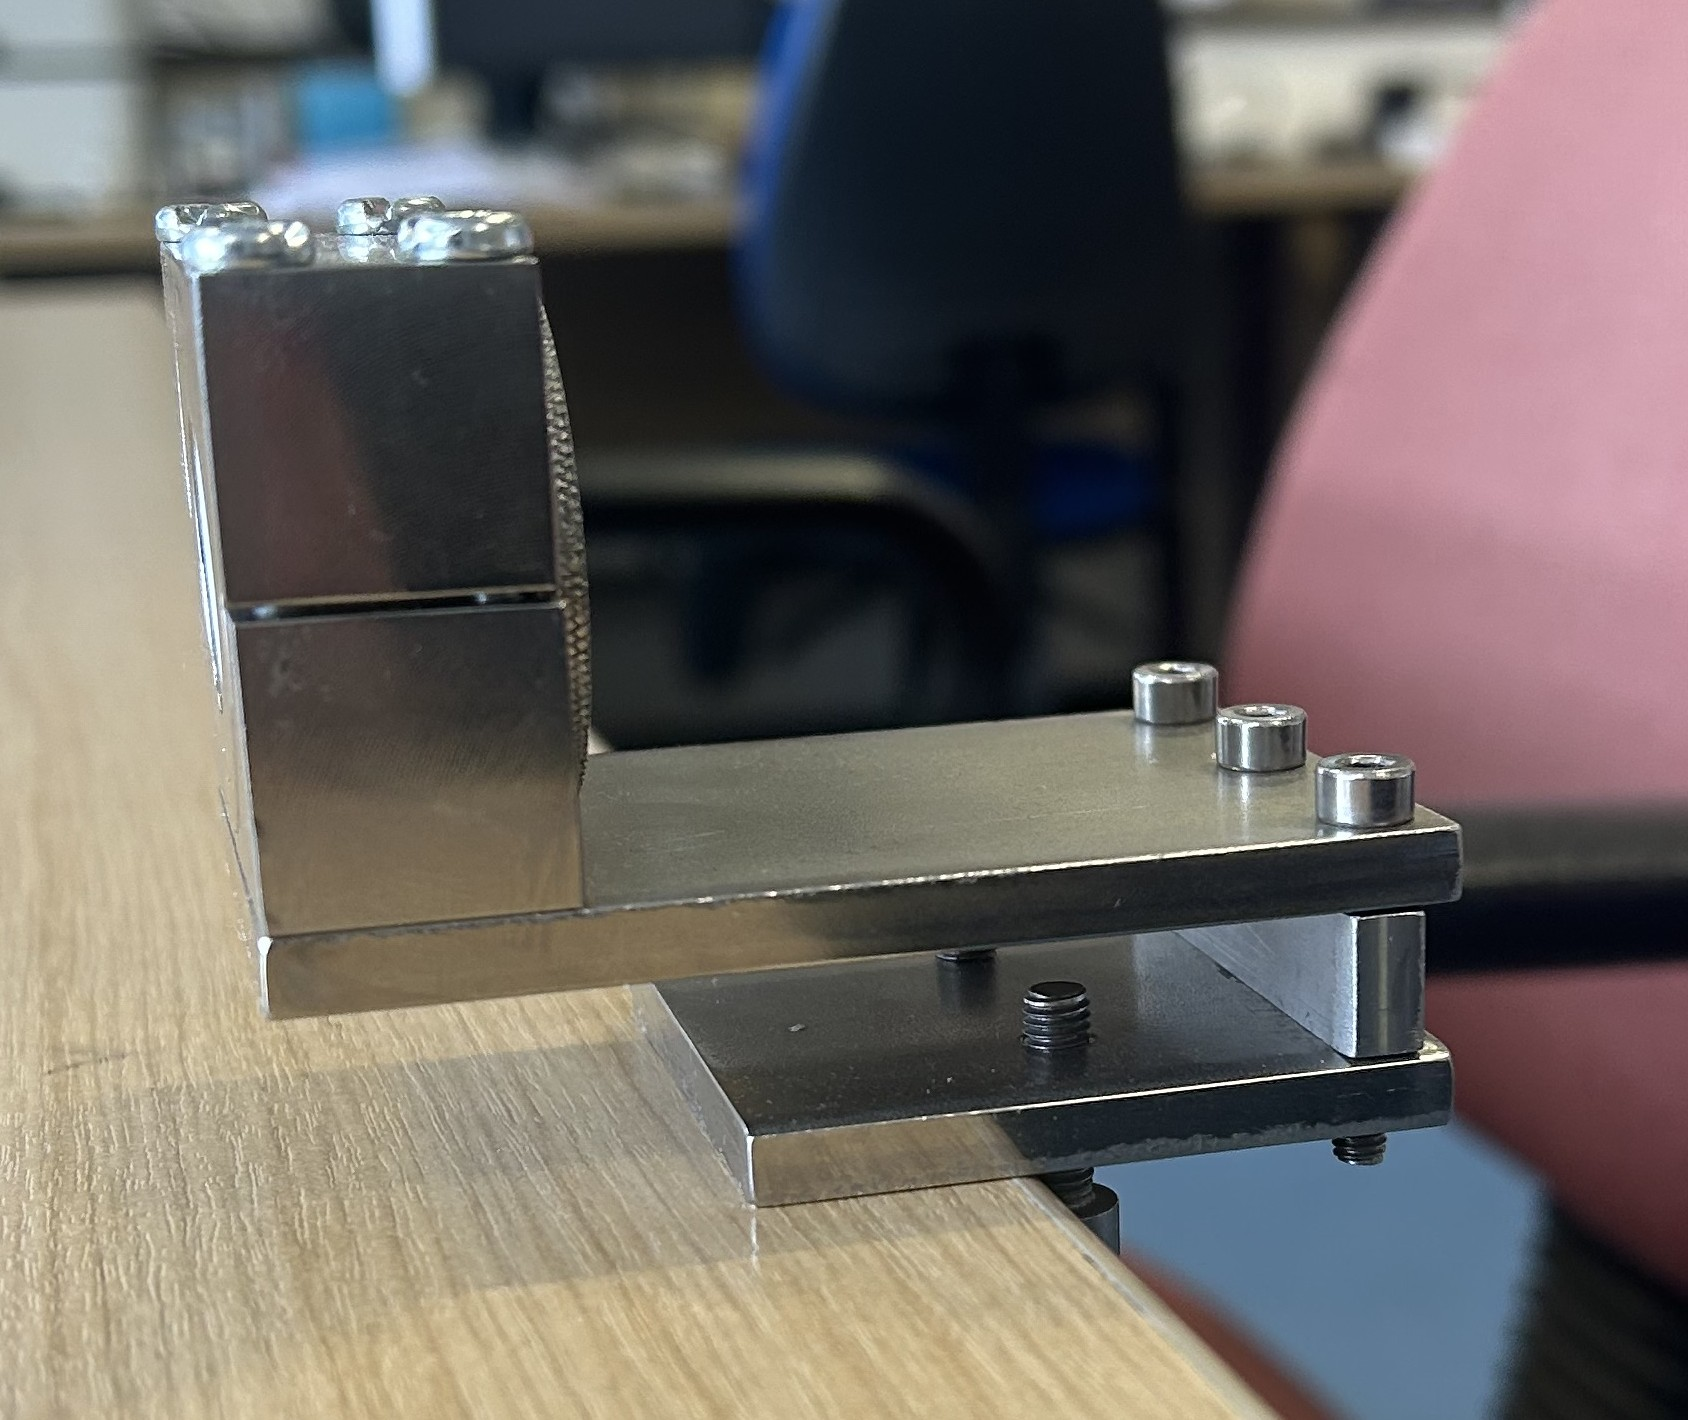
\includegraphics[width=.45\textwidth]{OD_stand_tophat_side.jpg}%
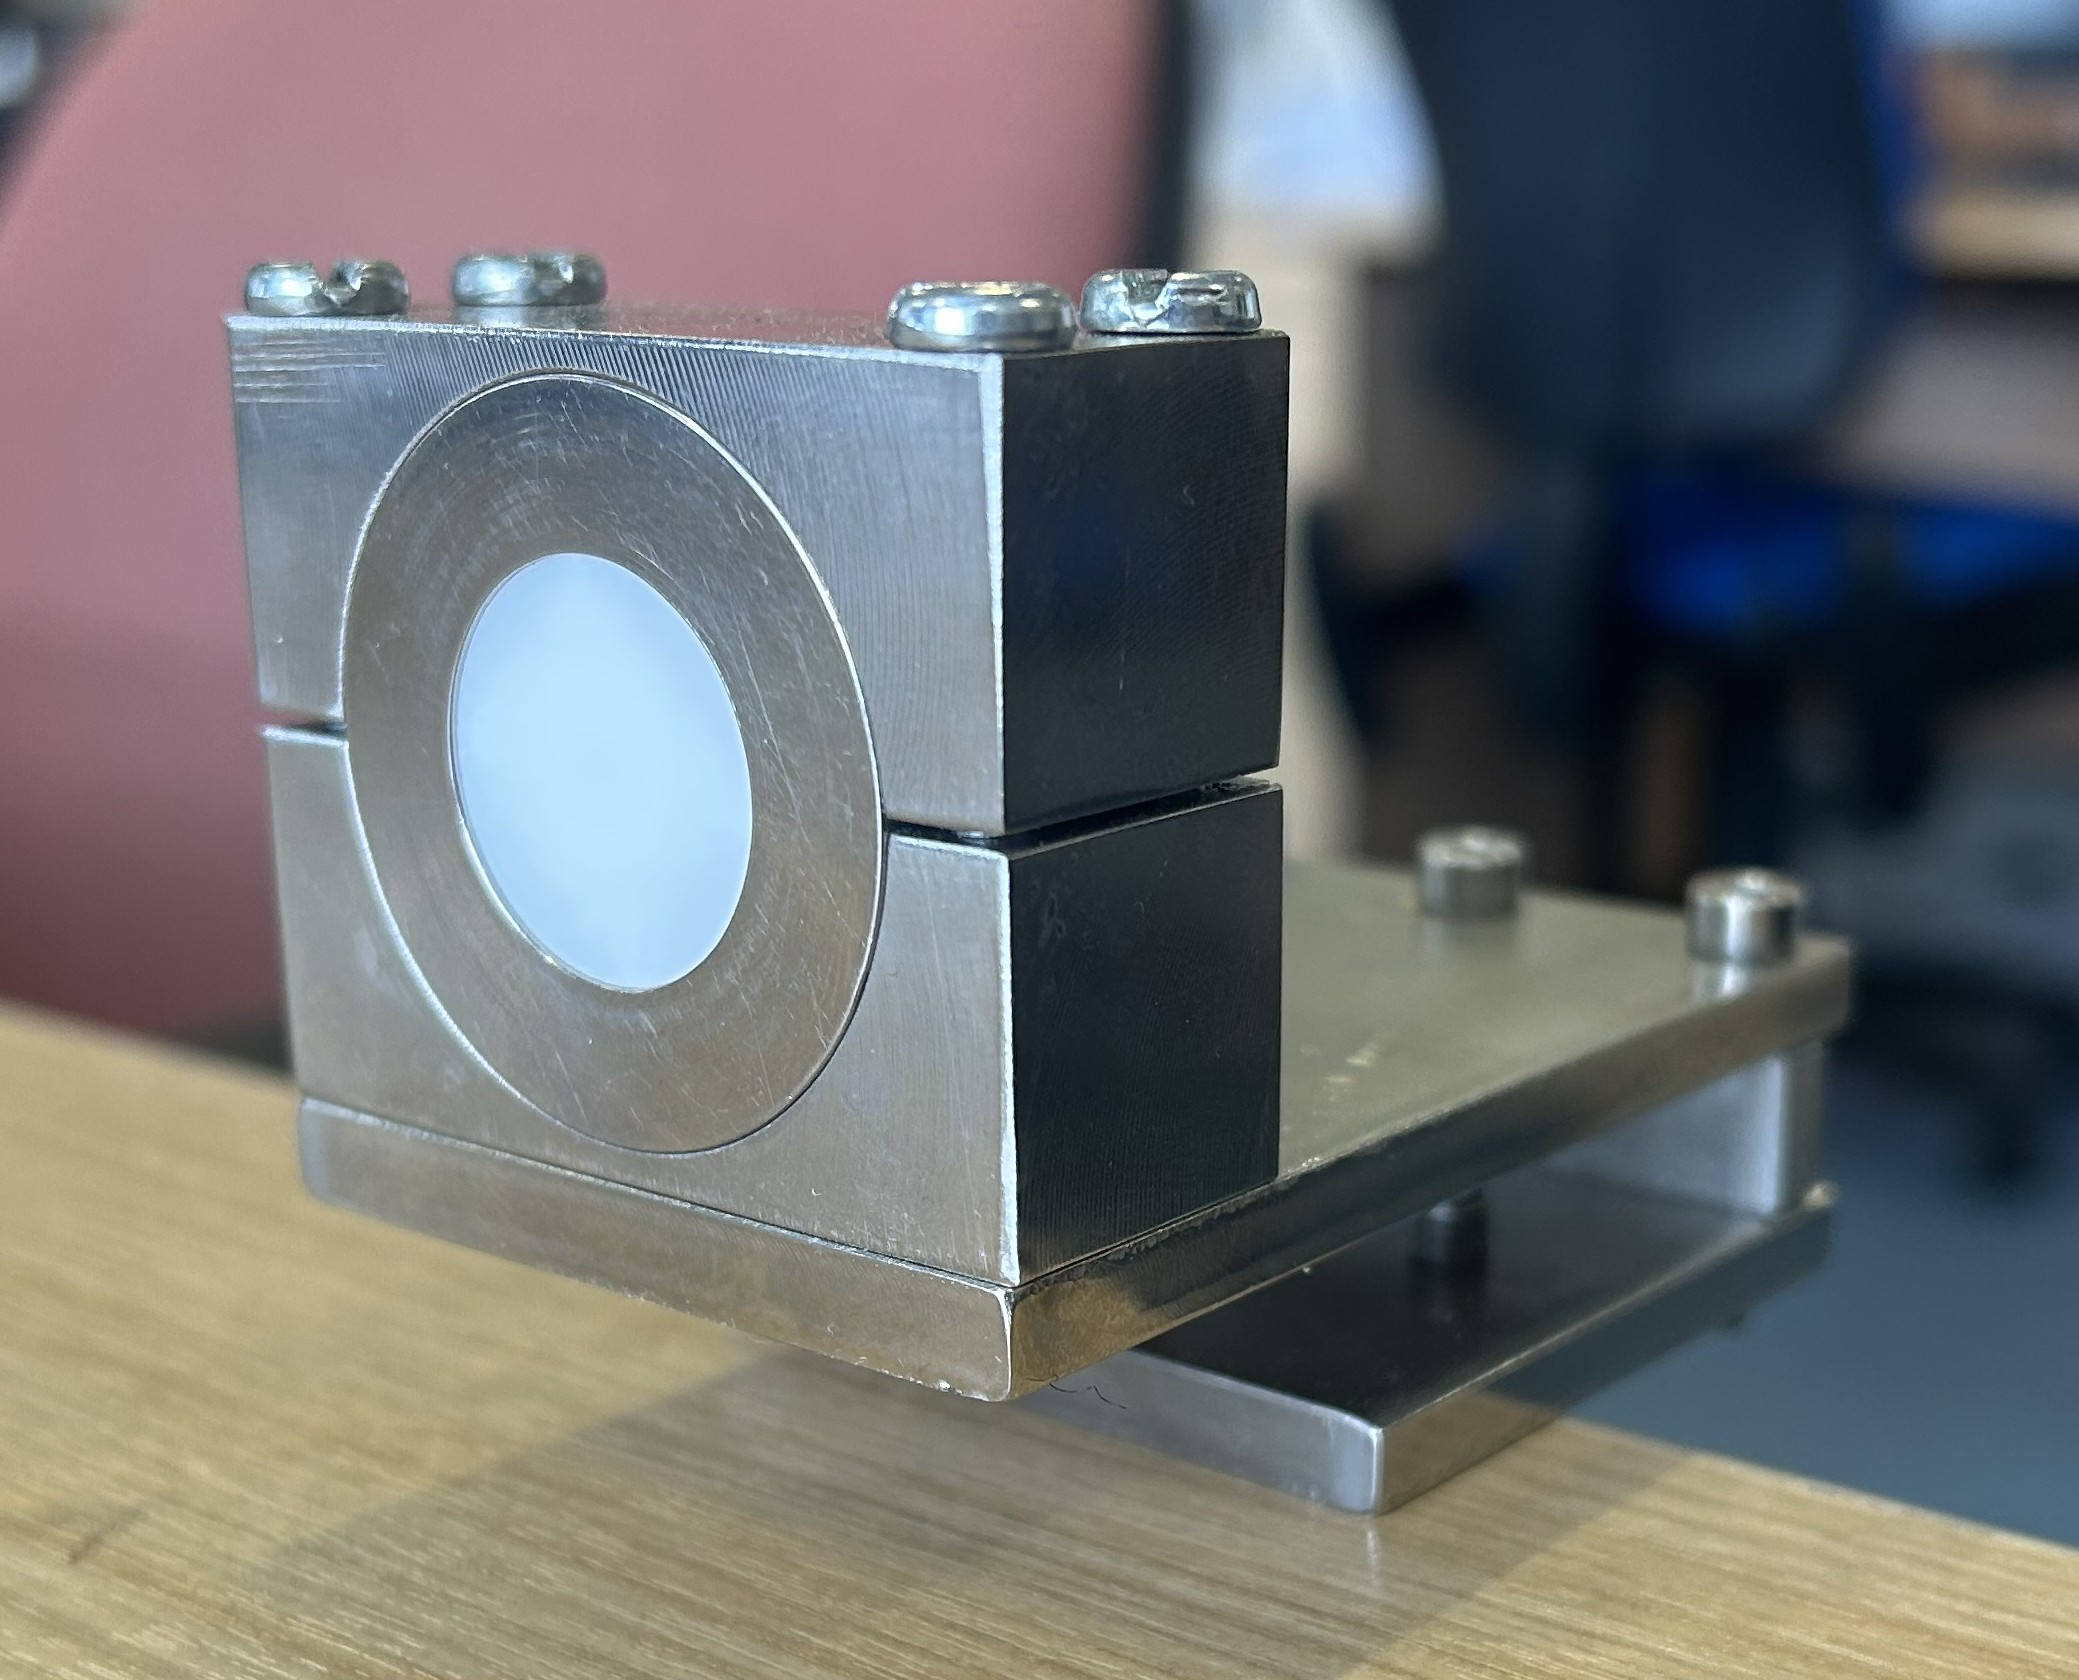
\includegraphics[width=.45\textwidth]{OD_stand_tophat_front.jpg}
\caption{(left) Side view of the prototype holder and (right) front view of the prototype holder.}
\label{fig:od_diffuser_mount_pics}
\end{figure*}

Drawings for the OD diffuser prototype mount can be seen in \cref{fig:od_diffuser_mount} and pictures of the prototype can be seen in \cref{fig:od_diffuser_mount_pics}. The mount is made from stainless steel and is designed to hook over a horizontal frame bar, and screw in from the bottom. The PTFE mount is approximately 5 cm on a side. The fibre will be installed from the back and is held in place by a T-shaped component that is screwed down by the gondola worker.


\section{Pulser Board}\label{sec:LEDpulser}

\subsection{Pulser Board Overview}

The pulser board was designed to be a more efficient and compact version compared to Super-Kamiokande UK Light Injection system, improving on efficiency, functionality, and light output. The pulser board is a rather simple board designed for low cost production. This section explains each circuit, component selection and design decision. As of writing, the board development is v0.9. v1.0 will be ready by September and will have only minor changes and adjustments compared to v0.9, mostly centered on refinement and removing the prototyping circuit. 


\subsection{Physical dimensions and construction}

The dimensions of the Printed Circuit Board (PCB) were selected to be as compact as practicable, while still providing sufficient area for the secure mounting of a fibre coupler and for the components. The final board size is 50~mm~$\times$~30~mm. This configuration permits electrically noisy components, such as switching power supplies and the Low Voltage Differential Signal to Transistor Transistor Logic (LVDS-to-TTL) converter to be positioned at a maximum distance from the switching circuitry, thereby minimising potential electromagnetic interference.

Although it is technically feasible to further reduce the board size, preliminary design studies and practical build indicated no substantial benefit in doing so. The board density cannot be significantly increased inside the crate due to  FPGA LVDS count and Eurocard dimension, and cost analyses revealed negligible differences associated with a smaller PCB footprint. Furthermore, the chosen dimensions provide an adequate area for the fibre coupler and the necessary mounting holes to affix the pulser board onto the Eurocard, thereby ensuring reliable optical alignment and mechanical stability.
The PCB is fabricated as a four-layer FR4 \cite{FR-4}  board with a thickness of 0.8~mm, in accordance with the standard construction offered by PCB Train/Newbury Electronics\footnote{These are trading names of the same manufacturer.}, see \cref{fig:PCBTrain0.84layer}. Refer to \cref{fig:PulserBoard0.93DTopandBottom} for the 3D model of the pulser board. The Top Layer and Inner Top Layer are shown in \cref{fig:PulserBoard0.9TopLayers}, and the Inner Bottom Layer and Bottom Layer are likewise illustrated in \cref{fig:PulserBoard0.9BottomLayers}. A combined view of all PCB layers is provided in \cref{fig:PulserBoard0.9Overview}.


\begin{figure}[htbp]
\centering
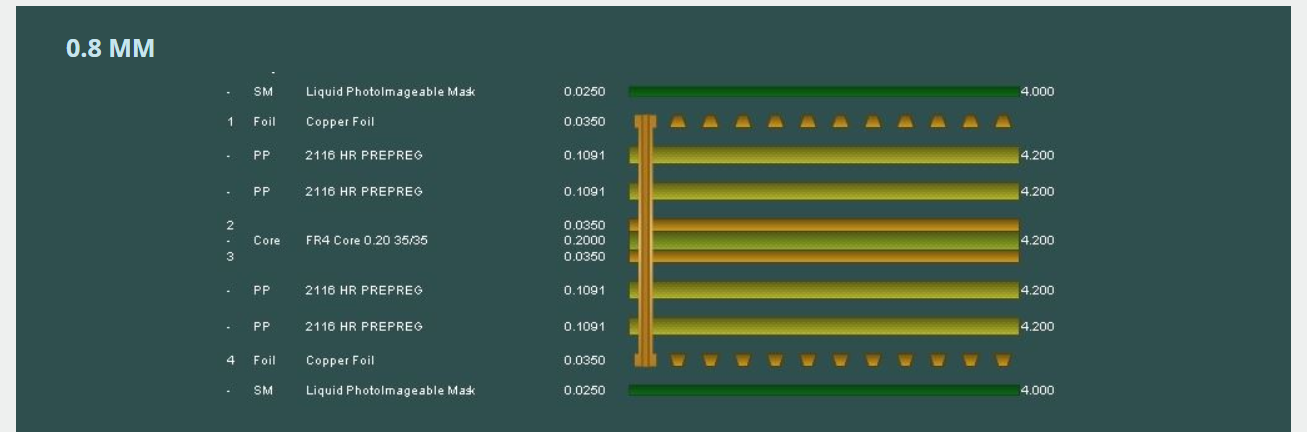
\includegraphics[scale=0.5]{PCBTrain0.84layer.png}
\caption{PCB Train's 4 Layer 0.8mm Layer Stack\label{fig:PCBTrain0.84layer}}
\end{figure}

\begin{figure}[htbp]
\centering
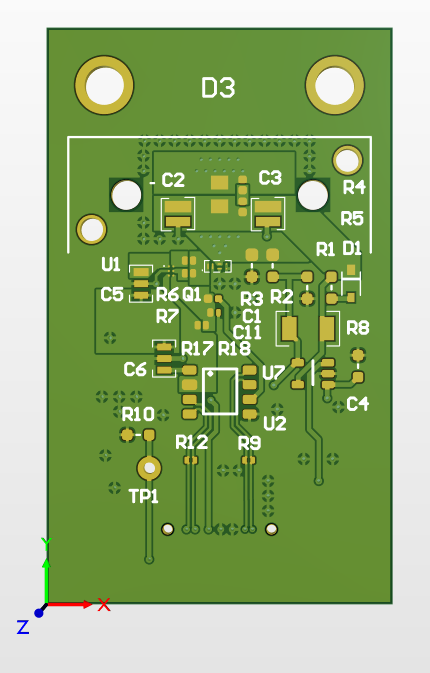
\includegraphics[scale=0.5]{PulserBoard0.93DTop.png}
\qquad
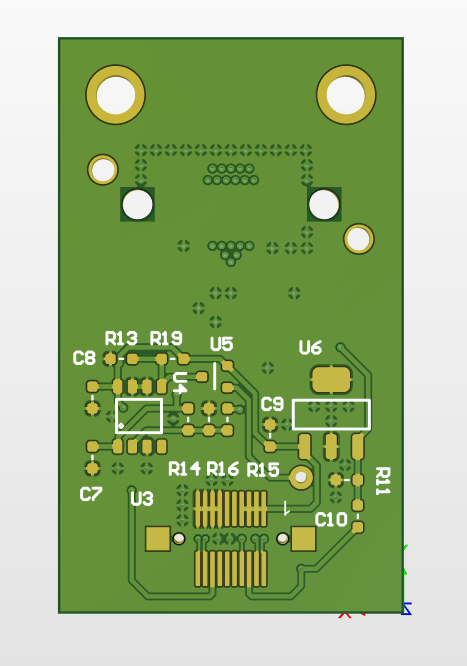
\includegraphics[scale=0.5]{PulserBoard0.93DBottom.png}
\caption{Pulser Board's 3D view Top and Bottom\label{fig:PulserBoard0.93DTopandBottom}}
\end{figure}

\begin{figure}[htbp]
\centering
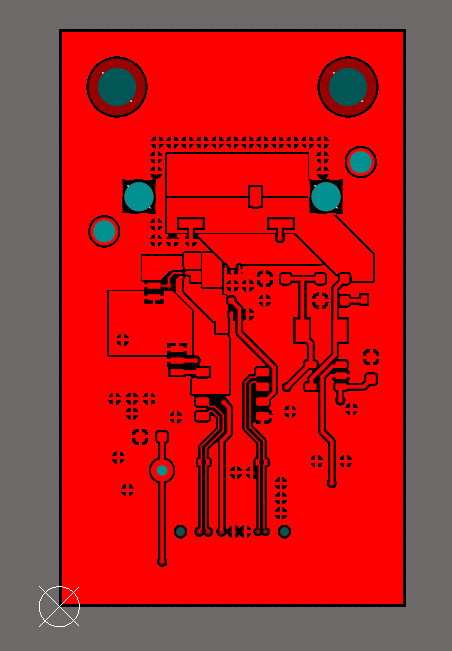
\includegraphics[scale=0.5]{PulserBoard0.9TopLayer.png}
\qquad
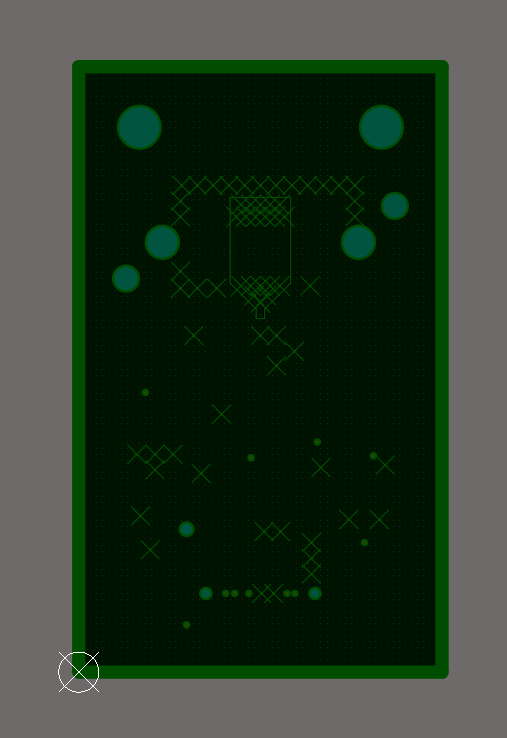
\includegraphics[scale=0.5]{PulserBoard0.9InnerTopGround.png}
\caption{Pulser Board Top and Inner Top Layer\label{fig:PulserBoard0.9TopLayers}}
\end{figure}

\begin{figure}[htbp]
\centering
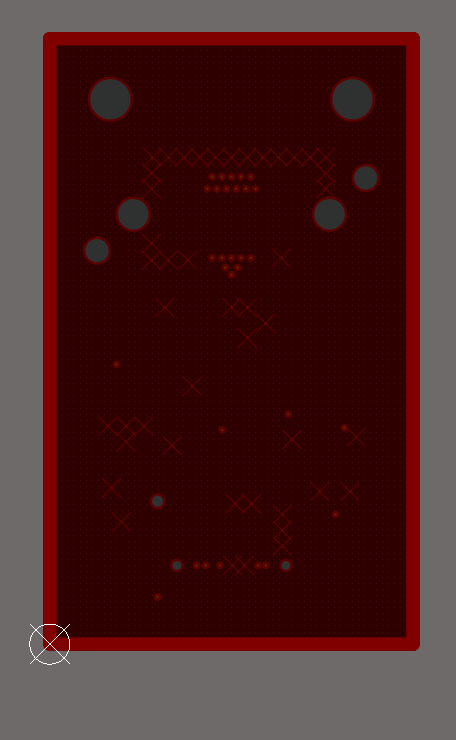
\includegraphics[scale=0.5]{PulserBoard0.9InnerBottomLayer.png}
\qquad
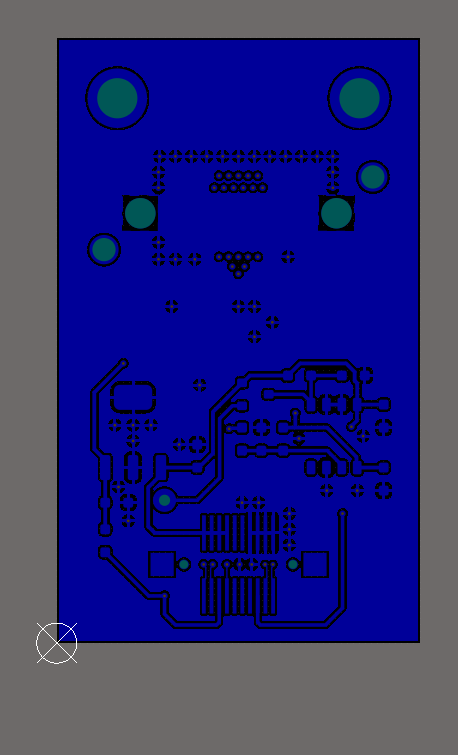
\includegraphics[scale=0.5]{PulserBoard0.9BottomLayer.png}
\caption{Pulser Board Inner Bottom and Bottom Layer\label{fig:PulserBoard0.9BottomLayers}}
\end{figure}


\begin{figure}[htbp]
\centering
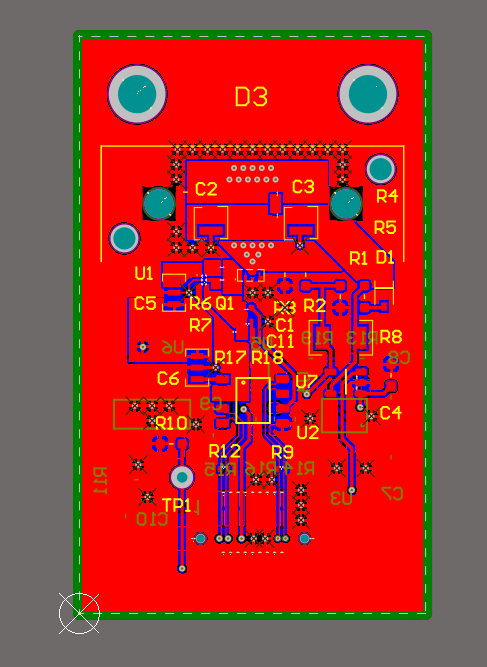
\includegraphics[scale=0.5]{PulserBoard0.9Overview.png}
\caption{Pulser Board Layer Overview\label{fig:PulserBoard0.9Overview}}
\end{figure}

\subsection{LED}

\subsubsection{Overview}

The LEDs are the most crucial component in the system as the characteristics of these primarily determine the light output, regardless of electronics. LEDs are usually not rated for such high-speed applications, which meant LEDs had to be tested and validated in-house, as datasheets do not provide the required information. The specification required was a 1--10~ns clean single pulse, sub-400 nm wavelength, small surface mount package, narrow output beam so it can be coupled to a fibre with reduced losses and a good range of photon output. Several LED packages were purchased from Kingbright and LC-LED, and their performance tested. The results of these tests are given in \cref{sec:LEDtesting}.

%sort the part numbers out



\subsubsection{Switching Circuit}


The redesign process provided a valuable opportunity to evaluate a revised layout and new components for the switching circuit. Several enhancements have since been implemented in the revised switching circuit. Most importantly, the switching side of the layout has been rerouted. In contrast to the previous configuration, where current would flow through the limiting resistor regardless of the LED state, the updated design only allows current flow when the LED is active (refer to \cref{fig:Switching circuit}). This modification reduces both thermal dissipation and the overall power consumption of the system.
To modulate light intensity, a variable power supply is now employed to adjust the voltage supplied to the LED. This method has proven highly effective. Tests were conducted at various voltage levels using the full 181~m length of optical fibre—the maximum expected in Hyper-K at the time of testing—and the resulting photon output ranged from approximately $1\times10^5$ to $2\times10^7$ photons per pulse. Refined testing results are shown in \cref{sec:LEDtesting}.
Further discussion regarding the implementation and performance of the variable voltage supply is provided in \cref{sec:LEDpower}.


\begin{figure}[htbp]
\centering
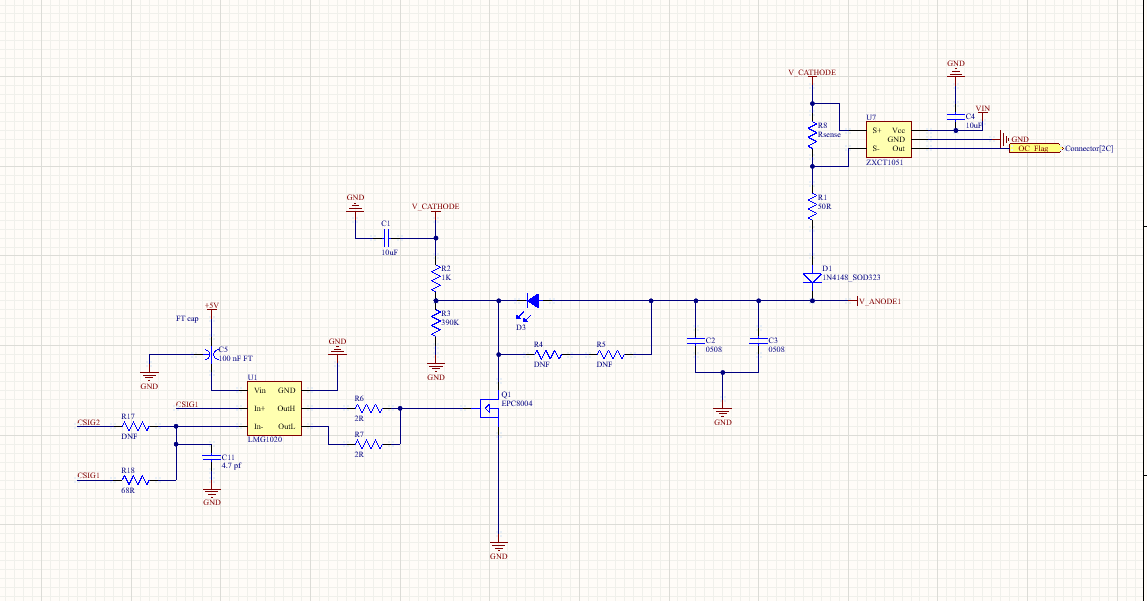
\includegraphics[scale=0.5]{Switching circuit.png}
\caption{Switching Circuit Layout with LMG1020 and over current IC, R4 is 6.8~nH inductor and R5 is 3R3 resistor\label{fig:Switching circuit}}
\end{figure}


\subsubsection{Switch Selection}

The previous iteration of the pulser board utilised a BFR92 \cite{BFR92} high-speed RF NPN switching transistor which was directly driven by a LVDS-to-TTL converter. In the redesign phase, alternative circuit topologies were explored—particularly those suitable for generating (sub-)nanosecond pulses. This investigation led to the adoption of gate driver circuits. Gate drivers are advantageous not only because they can power switches with challenging drive requirements, but also because sub-nanosecond electrical pulses can be achieved by modulating the enable pin with slight timing offsets.

The fastest commercially available gate driver identified was the Texas Instruments LMG1020 \cite{LMG1020}. This device supports pulse widths down to 1~ns, with typical rise and fall times of 400~ps. Additionally, it features an enable pin that allows for precise nanosecond pulse shaping \footnote{See page 12 and 13 in \cite{LMG1020}.}. The LMG1020 is compatible with both Gallium Nitride Field Effect Transistor (GaN) and Metal Oxide Semiconductor Field Effect Transistor (MOSFET) switches, broadening the scope for future component integration and experimentation. It is widely available and priced at £1.97 per unit in the quantities we will require for full production.

For the switching element, enhancement-mode GaN transistors manufactured by EPC were selected due to their superior switching characteristics. This recommendation originated from Nick Braam, an engineer at the University of Victoria, who contributed to the pulser board design for the mPMT system. Two EPC devices were shortlisted: the EPC2012 \cite{EPC2012} and EPC8004 \cite{EPC8004}. The EPC2012 offers a simpler footprint, which could reduce manufacturing defects. However, the EPC8004 features lower parasitic capacitance, see \cref{fig:EPC2012Cap} for the EPC2012 values and \cref{fig:EPC8004Cap} for EPC8004 values, leading to better high-speed performance.

To evaluate optical output performance, a 40~m length of FP400URT \cite{FP400URT} optical fibre, a Mouser-sourced 385~nm LED (ATS2012UV385 \cite{ATS2012UV385}), and a Hamamatsu H10721-210 \cite{H10721-210} PMT were used. The EPC-based configurations exhibited nearly identical pulse shapes, whereas the BFR92-based circuit's pulse shape was less sharp at identical pulse widths, as shown in \cref{fig:BFR92PulseShape}. Consequently, the EPC8004 (\cref{fig:EPC8004PulseShape}) was chosen for implementation. Optimal performance of the EPC GaN switches required careful layout considerations. A layout was developed in accordance with EPC's design guidelines \cite{EPCHSGuide}, targeting minimal parasitic inductance and capacitance. The design employs two layers placed directly above one another, utilising large copper planes and multiple vias to ensure uniform current distribution. The PCB will be fabricated and assembled by PCB Train, using their 0.8~mm thick, four-layer stack-up, which offers minimal inter-layer separation for optimal electrical performance (\cref{fig:PCBTrain0.84layer}). This same layout strategy was applied to the BFR92 circuit to provide a fair performance comparison.

A significant challenge at low pulse widths is the presence of a trailing edge or “tail” in the LED output. This effect arises due to charge accumulation and the intrinsic capacitance of the LED, resulting in extended decay times and pulse broadening (see \cref{fig:NoRLPulse}). To mitigate this, a parallel modified snubber circuit was implemented, consisting of a 6.8~nH inductor and a 3.3~$\Omega$ current-limiting resistor. Upon LED turn-off, the inductor generates an electromotive force (EMF) that actively extracts residual charge from the LED, accelerating its shutdown. The effectiveness of this approach is illustrated in \cref{fig:RLPulse}.
Additionally, two 0508 reverse-topology 100~nF capacitors have been incorporated. Their role is to act as local energy reservoirs, providing rapid current delivery to the LED during pulse operation, surpassing the response time of the main power supply.

\begin{figure}[htbp]
\centering
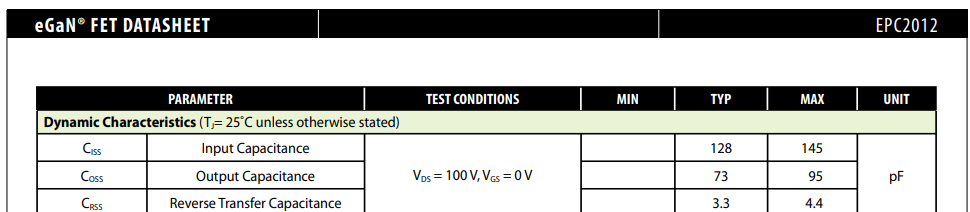
\includegraphics[scale=0.8]{EPC2012Cap.png}
\caption{EPC2012 Capacitance Values IC\label{fig:EPC2012Cap}}
\end{figure}

\begin{figure}[htbp]
\centering
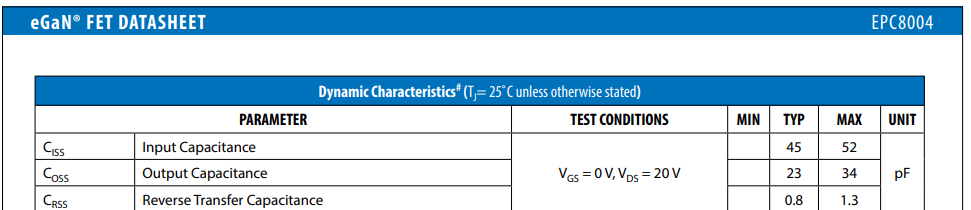
\includegraphics[scale=0.8]{EPC8004Cap.png}
\caption{EPC8004 Capacitance Values IC\label{fig:EPC8004Cap}}
\end{figure}

\begin{figure}[htbp]
\centering
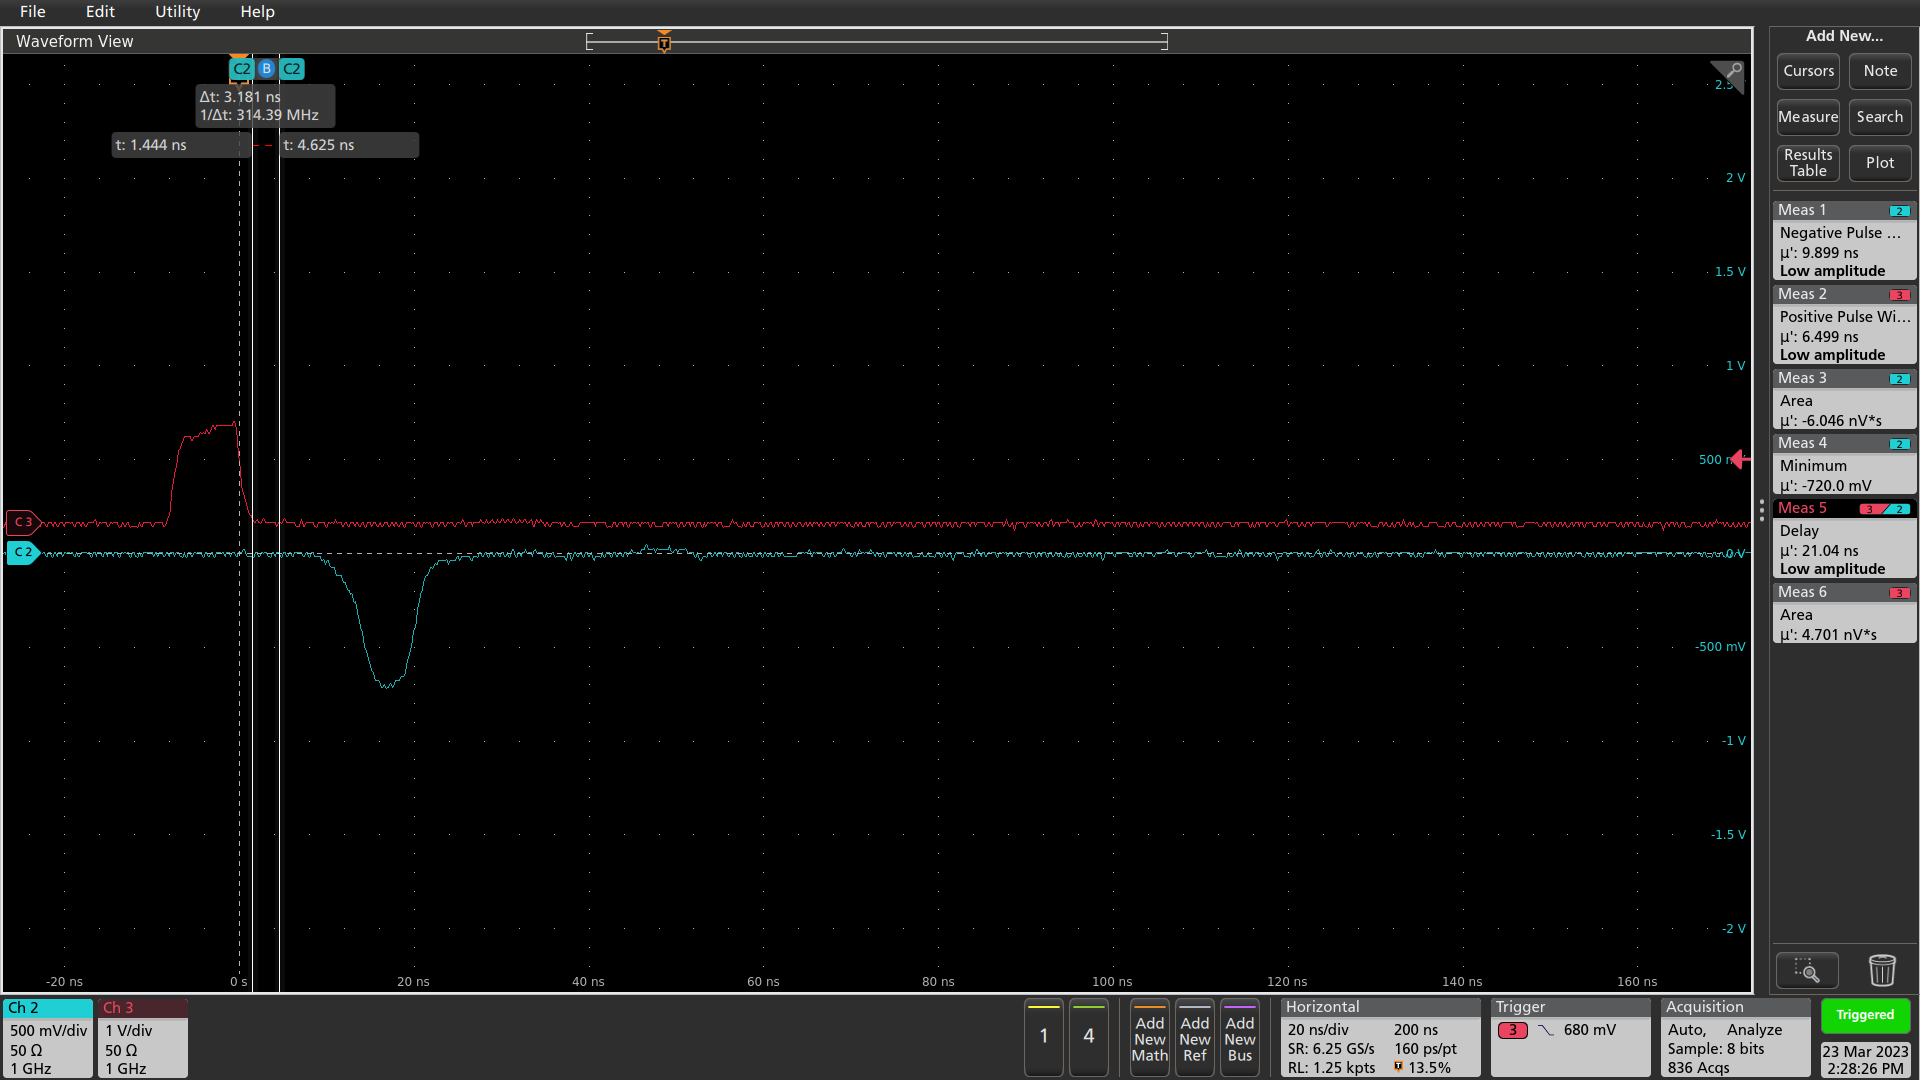
\includegraphics[scale=0.3]{bfr92st310nh_000.png}
\caption{BFR92 Pulse Shape\label{fig:BFR92PulseShape}}
\end{figure}

\begin{figure}[htbp]
\centering
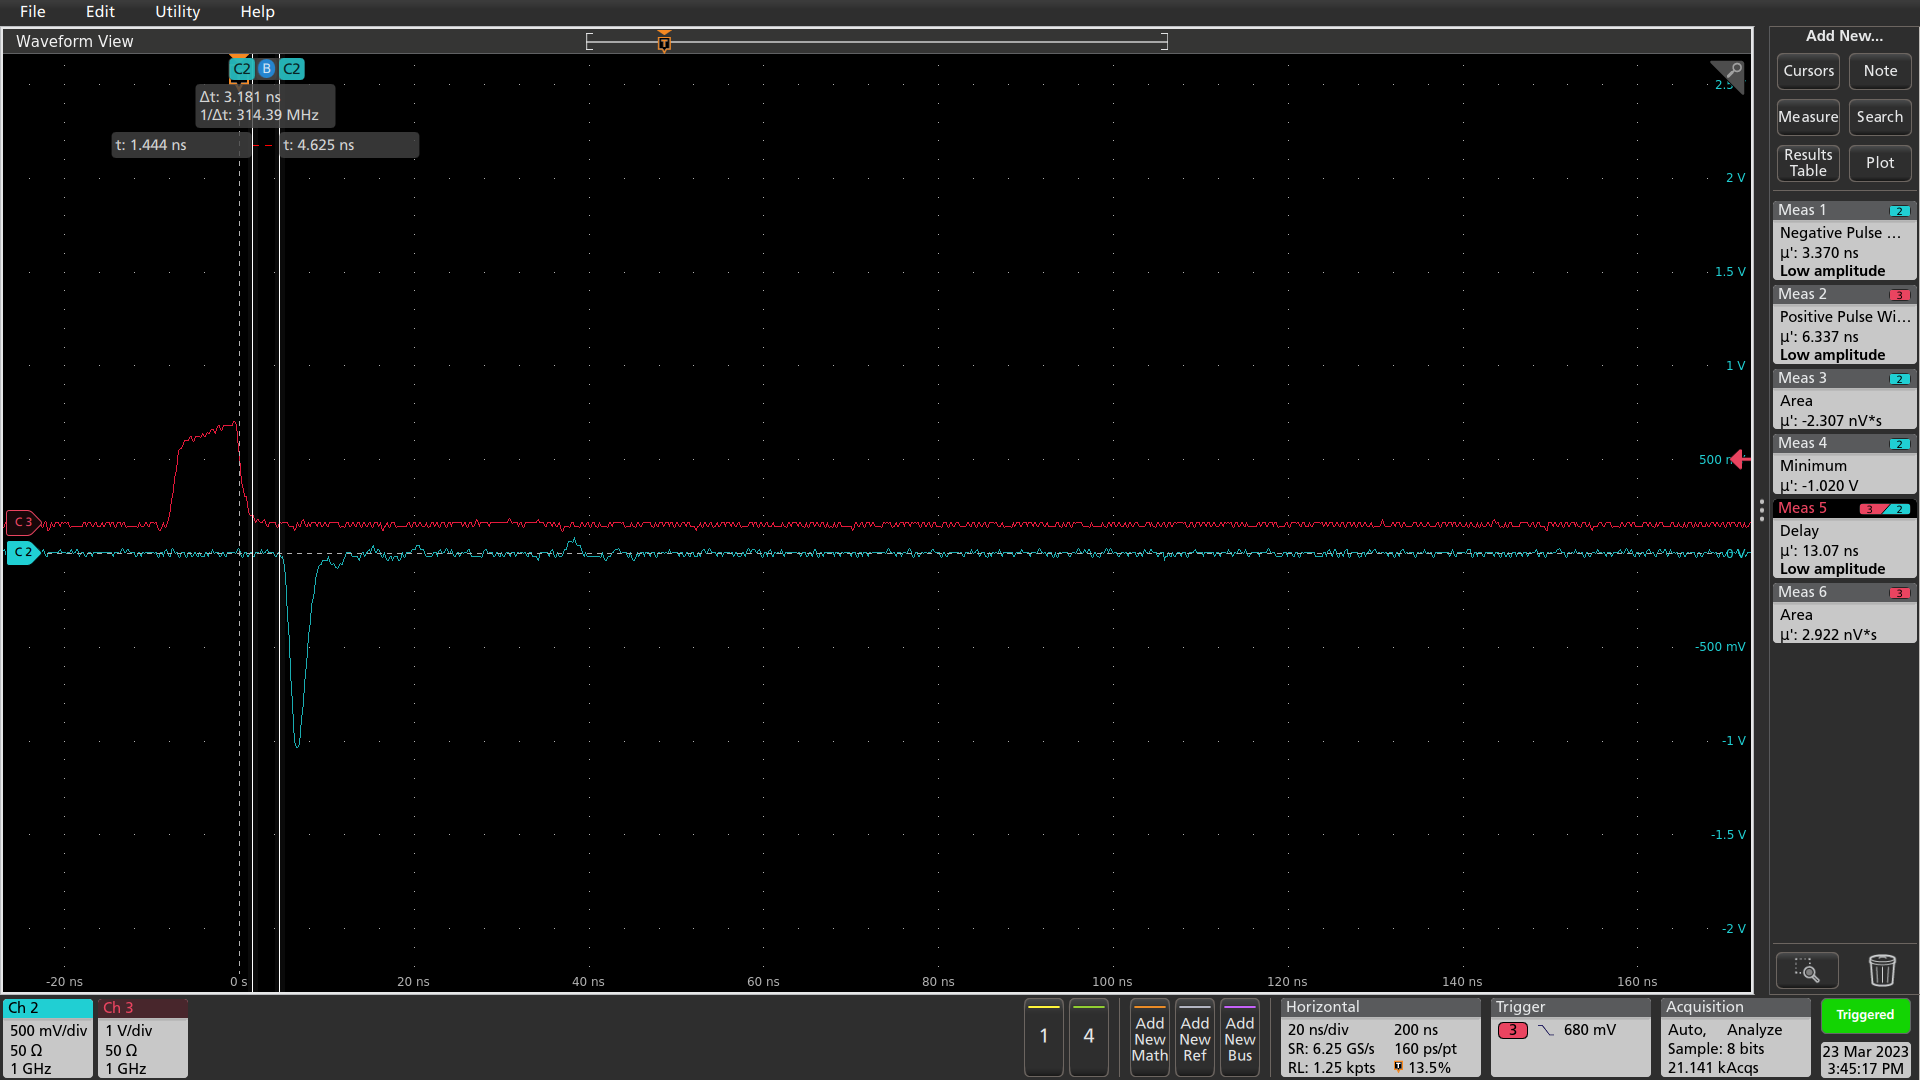
\includegraphics[scale=0.3]{800420nh47pf_000.png}
\caption{EPC8004 Pulse Shape\label{fig:EPC8004PulseShape}}
\end{figure}

\begin{figure}[htbp]
\centering
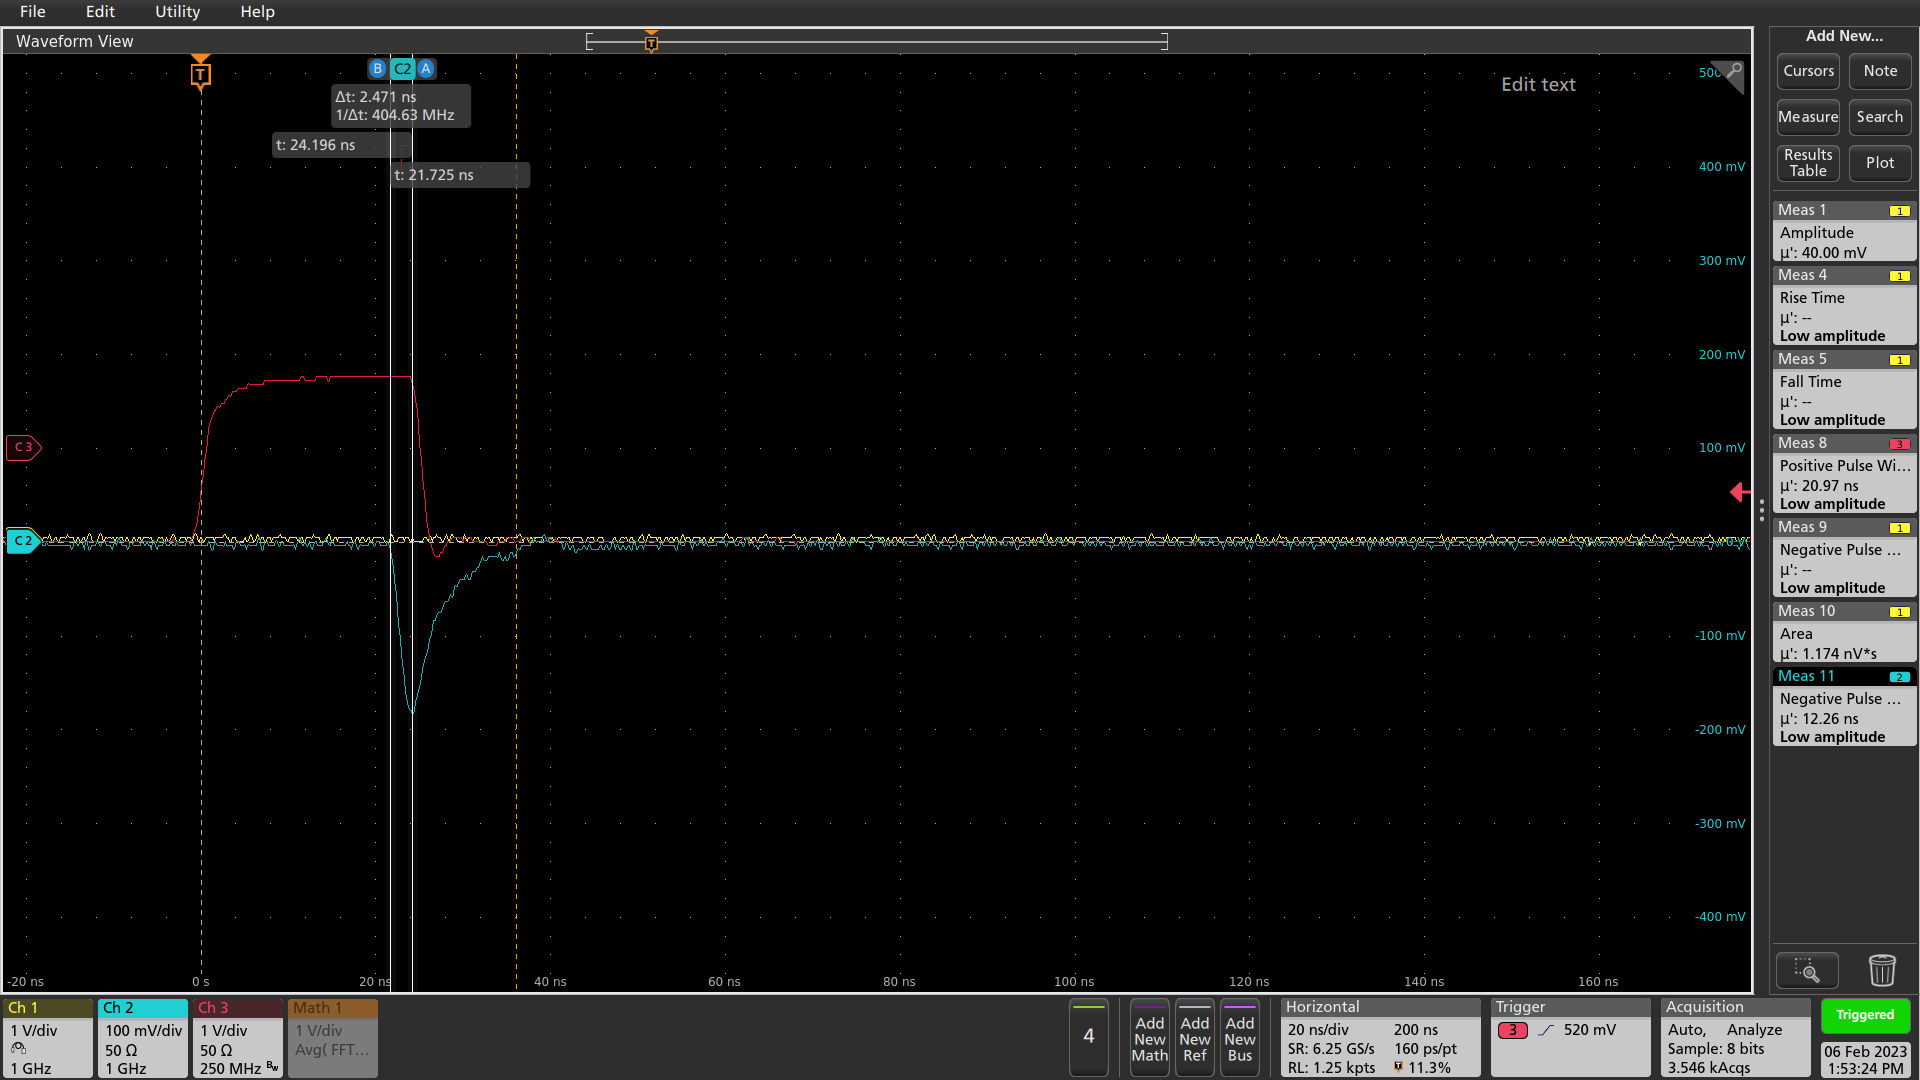
\includegraphics[scale=0.3]{RCTHTest1 no inductor.png}
\caption{Pulsing Circuit With No Inductor and Resistor\label{fig:NoRLPulse}}
\end{figure}

\begin{figure}[htbp]
\centering
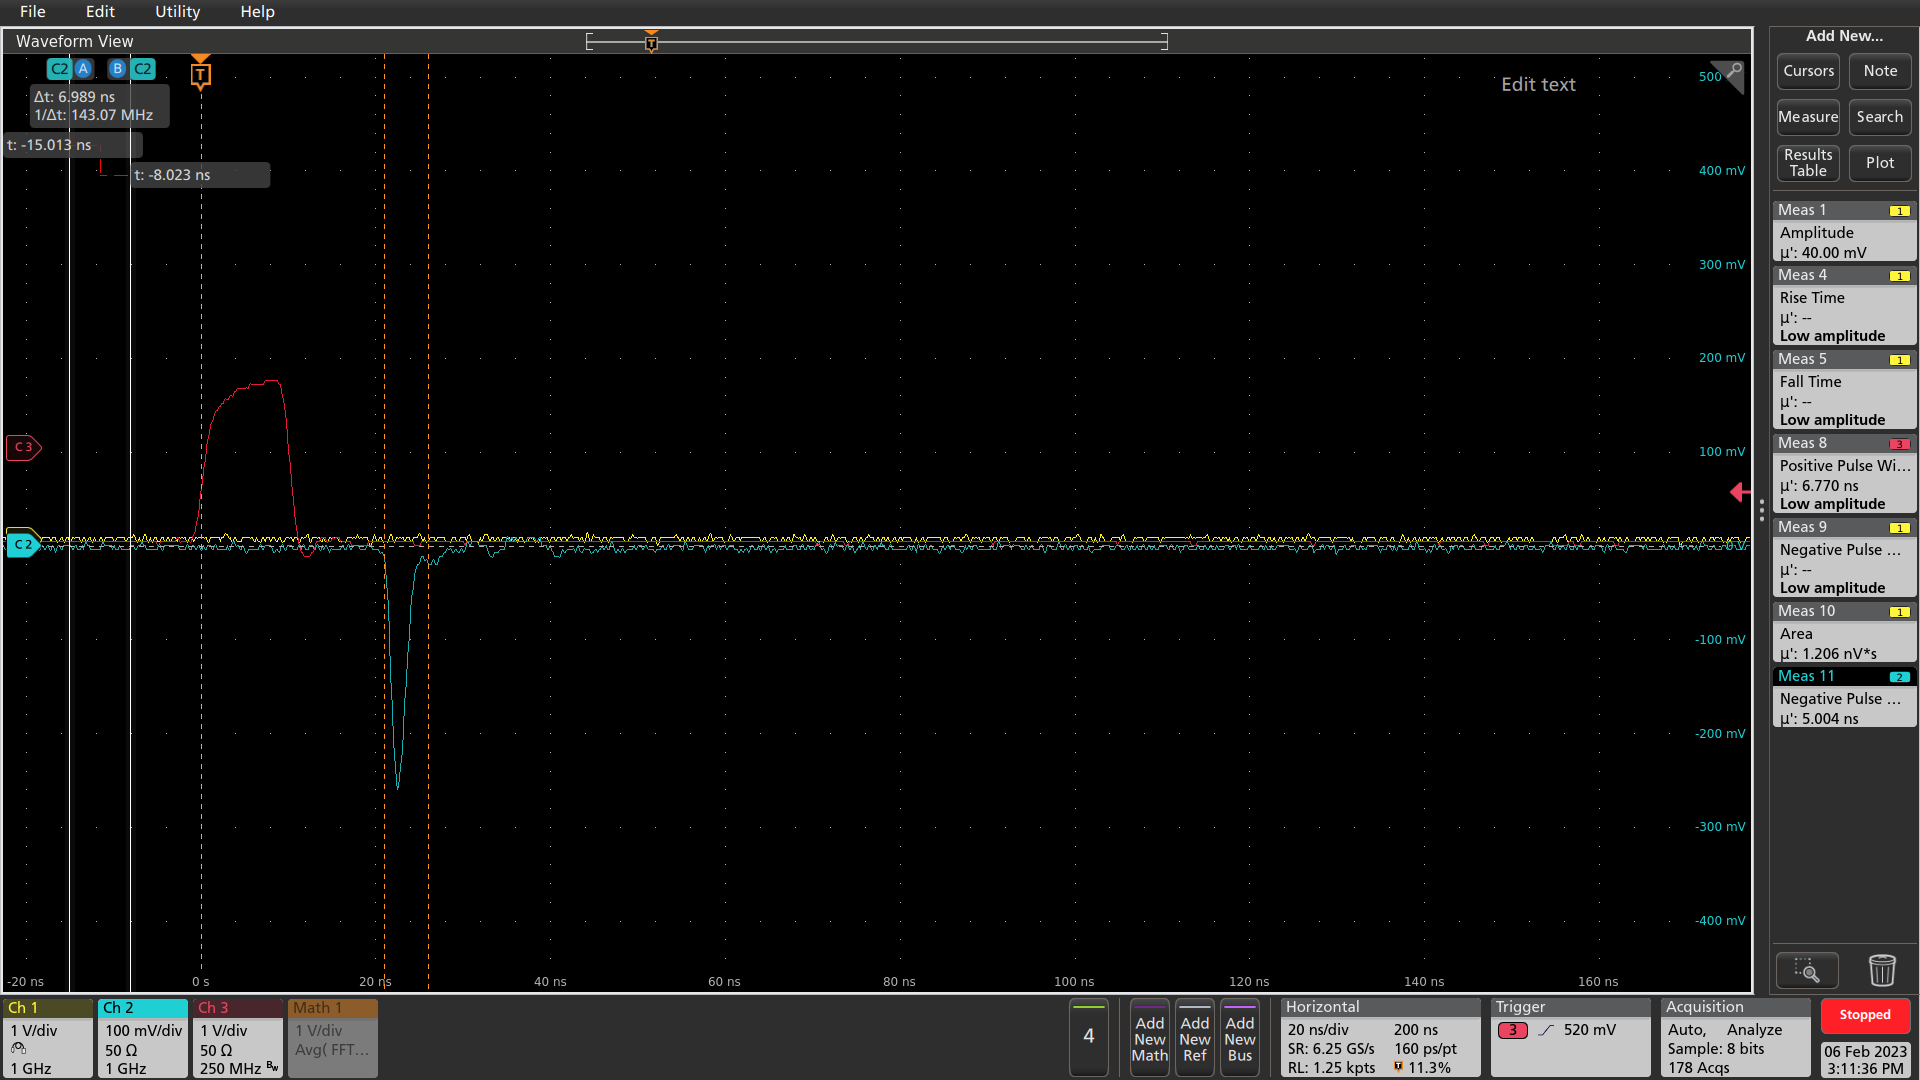
\includegraphics[scale=0.3]{RCTHTest1 inductor circuit.png}
\caption{Pulsing Circuit With Inductor and Resistor\label{fig:RLPulse}}
\end{figure}

%Check for diikey LED, that will will be in the future and check for LED part numbers
\subsubsection{Testing}\label{sec:LEDtesting}

For testing purposes, the previous-generation United Kingdom Light Injection (UKLI) motherboard and associated software were utilised in conjunction with a prototype of the next-generation pulser board. This prototype consisted of four distinct circuit variants: one employing the EPC8004 switch, another utilising the EPC2012 switch, a third using the same high-speed transistor (BFR92) as implemented in the legacy system, and a fourth variant incorporating an EPC2012 gate in a through-hole package instead of the standard 0805 surface-mount footprint. Further evaluation was also performed using the latest pulser board prototype once they had arrived.

Following comparative performance evaluations, the configuration using the EPC8004 switch was selected for continued use. While both the EPC8004 and EPC2012 switches exhibited similar electrical characteristics, the EPC8004 offered superior performance due to its lower parasitic capacitance, without any additional cost.
The pulser board assembly was housed within a dark box during testing, and a 3D-printed fibre coupler was employed to facilitate light delivery. The initial focus of the evaluation was on the shape of the generated optical pulse.
During component selection, it was observed that the LED previously sourced from Mouser (ATS2012UV385 by Kingbright) provided acceptable performance in terms of electrical characteristics, but the optical output was suboptimal. Additionally, this LED was found to be out of stock and obsolete at the time after testing, precluding further procurement. Subsequently, four ultraviolet LEDs from LC LED were assessed—two emitting at 365~nm and two at 395~nm—each in both 0805 and 0603 surface-mount packages. Results demonstrated that the 0805 package LEDs provided significantly better optical coupling efficiency with the FP400URT optical fibre. Furthermore, the 365~nm variant exhibited superior optical power output relative to the 395~nm counterparts.
Based on these findings, the LC LED UT-67UV365P~\cite{ut-67uv365p} 365~nm LED was selected as the most suitable LED for this application.



\subsection{LVDS to TTL Converter}

The DS90C402 \cite{DS90C402} from Texas Instruments was selected as the LVDS-to-TTL conversion solution. This device is a dual-channel converter, chosen primarily for its fast switching characteristics—offering both rise and fall times of approximately 500~ps. It operates at 5~V and provides 5~V TTL output levels, which aligns well with the requirements of the downstream switching circuitry. The inclusion of two channels is particularly advantageous, as it enables the generation of sub-nanosecond differential pulses by precisely offsetting the channels, as described in Switch Selection. Among commercially available devices with these specifications, the DS90C402 is the fastest and is readily available through multiple distributors.

The associated circuit was implemented in accordance with the manufacturer's recommendations provided in the datasheet. A decoupling capacitor was placed in close proximity to the power supply pin to minimise voltage ripple. Output traces were routed using polygon fills to reduce impedance and enhance signal integrity, and a continuous ground plane was placed beneath the signal layers to improve shielding and minimise electromagnetic interference. The schematic for this is given in \cref{fig:lvdsttl}.

\begin{figure}[htbp]
\centering
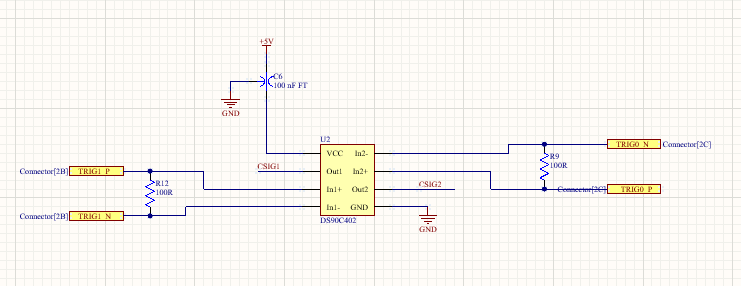
\includegraphics[scale=0.8]{LVDS-TTL Converter.png}
\caption{LVDS-TTL Converter Schematic\label{fig:lvdsttl}}
\end{figure}


\subsection{Power Supplies}\label{sec:LEDpower}

Each pulser board is required to incorporate a variable voltage power supply dedicated to driving the LED, with an adjustable output range from 3~V to 12~V. This supply is used exclusively to modulate the LED’s light output by varying the forward voltage, and consequently the current. The design specification also necessitates that the power supply be remotely controllable—i.e., capable of being switched on or off via a simple logic-level signal.

For this purpose, the LT1963A \cite{LT1963} adjustable low-dropout linear regulator was selected. This regulator has demonstrated reliable performance in previous pulser board iterations and offers a favourable balance of cost-effectiveness and controllability. The implementation includes standard filtering and decoupling, with layout details provided in \cref{fig:LT1963Layout}. The schematic provided in \cref{fig:12VVariablePSU} is an early version used for prototyping; the adjustable circuit has been simulated and will be tested shortly, and the enable circuit has been tested, modified and simplified. Updated schematics will be provided with v1.0 circuit.

\begin{figure}[htbp]
\centering
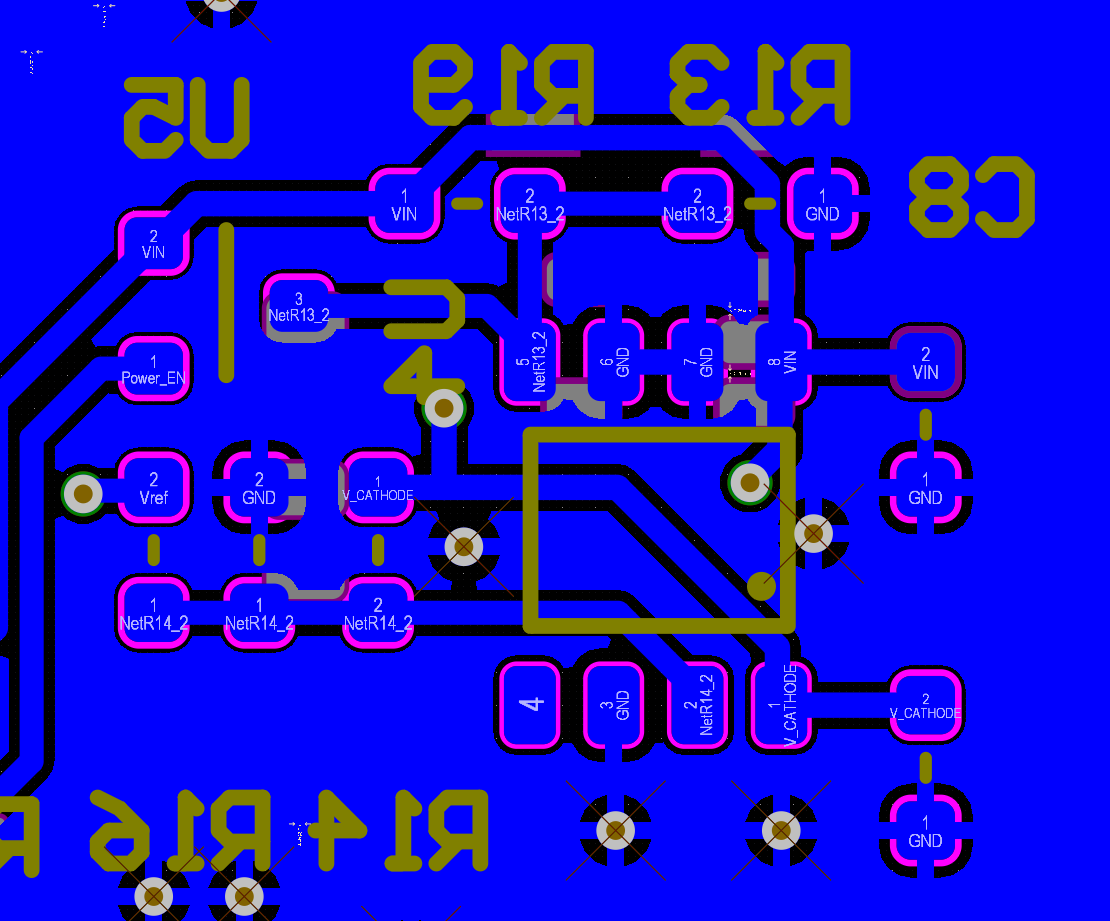
\includegraphics[scale=0.5]{LT1963layout.png}
\caption{LT1963 Layout\label{fig:LT1963Layout}}
\end{figure}

\begin{figure}[h]
\centering
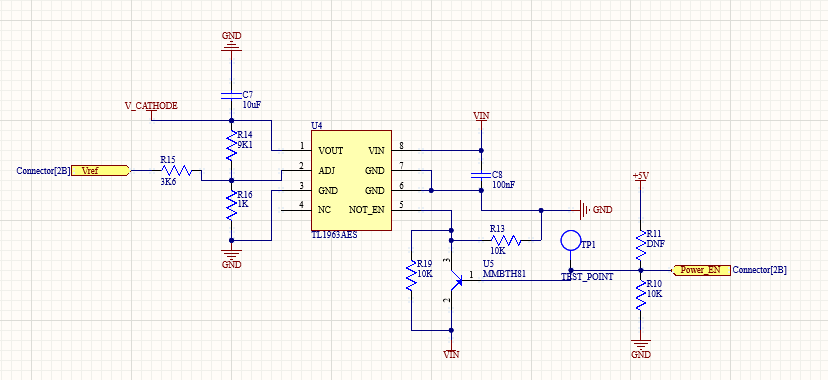
\includegraphics[scale=0.5]{12VVariablePSU.png}
\caption{12V Circuit Schematics\label{fig:12VVariablePSU}}
\end{figure}

In addition to the variable LED supply, each board requires a stable 5~V supply to power both the DS90C402 LVDS-to-TTL converter and the LMG1020 gate driver. Unlike the LED supply, this rail remains continuously powered. The 5~V supply is provided by an LM2937-5 \cite{LM2347-5}, a fixed-output linear voltage regulator, which has been successfully employed in various high-speed and low-noise applications within the laboratory. The associated circuit schematic and layout and schematic are shown in \cref{fig:LM29375Layout,fig:5VCircuit} respectively.

\begin{figure}[htbp]
\centering
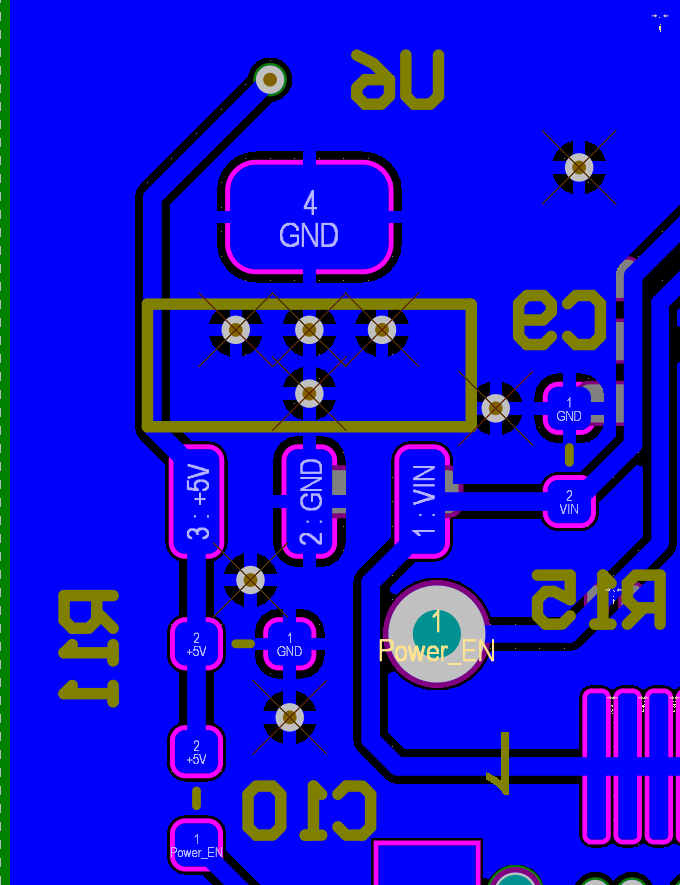
\includegraphics[scale=0.5]{LM29375Layout.png}
\caption{LM2937-5 Layout\label{fig:LM29375Layout}}
\end{figure}


To meet system-level design constraints, each pulser board is equipped with its own independent 12~V input supply, ensuring that LED output intensity can be individually controlled on a per-board basis. However, the 5~V supply is common across all boards and derived locally on each pulser module. This approach allows for localised filtering and minimal power distribution path lengths, reducing the risk of noise coupling and voltage drop considerations that are particularly critical in high-speed circuit applications.

Power is supplied to each board via the Eurocard backplane. The 12~V input from the Eurocard simultaneously feeds both the variable (LED) and fixed (logic) power regulators on the pulser board. The LED enable function is controlled via a 5~V logic signal originating from the Eurocard’s GPIO interface. Additionally, a DAC output from the Eurocard provides a voltage control signal to the adjustment pin of the LT1963A regulator on each pulser board, thereby allowing precise, programmable control of light intensity.


\begin{figure}[htbp]
\centering
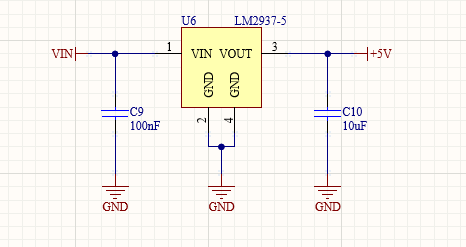
\includegraphics[scale=0.7]{5VCircuit.png}
\caption{5V circuit schematics\label{fig:5VCircuit}}
\end{figure}

\subsection{Connector}

The previous board connector was deemed too bulky and expensive for the larger number of channels needed in this system, leading to the process of finding a more suitable alternative. Following an evaluation of commercially available options, the Phoenix Contact female connector 1331962 \cite{1331962} was selected. This connector offers several advantageous specifications: it is rated for \SI{500}{\volt}, features a low contact resistance of \SI{40}{\milli\ohm}, supports a maximum current of \SI{0.5}{\ampere}, and is capable of signal transmission up to \SI{20}{\giga\bit\per\second}. In addition, it is cost-effective, priced at approximately \pounds 0.50 per unit, with wide availability ensuring ease of procurement. Multiple height variants are available within the same series, facilitating flexible mechanical integration within the Eurocard crate system. The compact footprint of the connector allows for a reduced PCB form factor. Electrically, the high-frequency performance supports reliable LVDS signal transmission. Additionally, the compact footprint of the connector is well-suited to space-constrained PCB layouts.

An illustration showing the connector and corresponding circuit layout is provided in \cref{fig:Connector}.

\begin{figure}[htbp]
\centering
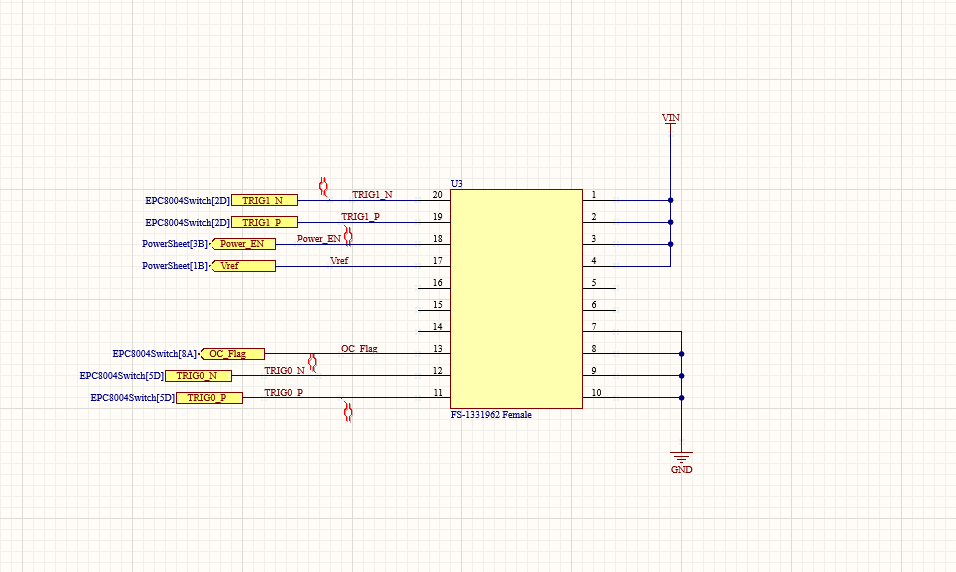
\includegraphics[scale=0.5]{Connector.png}
\caption{Connector Schematics\label{fig:Connector}}
\end{figure}


\subsection{Fibre Coupler}

During the prototyping phase, improvements were made to the PCB layout to better accommodate a fibre coupler. As a result, the current design includes provisions for precise mechanical mounting and alignment. Specifically, two mounting holes for M2 screws have been incorporated, enabling the 3D-printed coupler to be firmly secured to the board (see Figure~\ref{fig:OldFibreCouplerDesign}). In addition, two dowel holes have been added to guide the coupler into position, ensuring accurate alignment over the LED. Given the tolerances associated with PCB fabrication and 3D printing, an alignment accuracy of approximately \SI{100}{\micro\metre} is expected.

\begin{figure}[htbp]
\centering
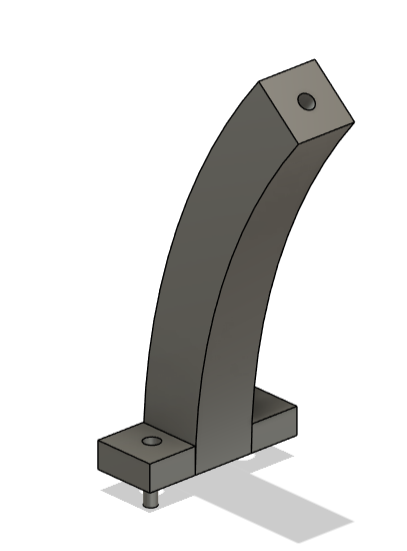
\includegraphics[scale=0.5]{OldFibreCouplerDesign.png}
\caption{Old Fibre Coupler Design\label{fig:OldFibreCouplerDesign}}
\end{figure}

To optimise the electrical path, capacitors have been repositioned as close as possible to the LEDs. This minimises parasitic inductance and resistance, while enabling a centralised layout of larger components. The resulting configuration creates a compact chamber housing both the LEDs and associated capacitors.

An earlier design for the fibre coupler, which assumed uniform fibre lengths for all channels, has since been abandoned. The current approach for the LED light injection system adopts five different fibre lengths, necessitating individual light attenuation for each channel. This attenuation will be implemented within the coupler itself, allowing the LED output to remain within the electronically controlled dynamic range.

The proposed design is modular, consisting of three components: a base section mounted to the pulser PCB, a top section into which the fibres will be epoxied, and an intermediate attenuator element. The latter will serve to space the fibre from the LED and thereby adjust the optical coupling efficiency to achieve the required attenuation. While an initial prototype will be developed in the near term for functional testing, the full design and validation of the fibre coupler will be undertaken later, once the required fibre lengths are fixed and unlikely to change. Should the project timeline require faster iteration, this can be pursued.

The fibre coupler will be fabricated via stereolithography (SLA) using a black resin to minimise light transmission through the material. Additional light-tight testing will be conducted, and black paint may be applied if further sealing is required. Furthermore, laser-cut rubber gaskets will be introduced at interface points to ensure optimal optical isolation and mechanical sealing.

\subsection{Photon Yield Tests}
{\color{red} tests on maximising photon yield and available dynamic range should be fully described here}

\subsection{Production}

Production will be carried out using PCB Train as they are local and competitively priced, and known to produce boards of good quality. Estimated cost is £12.27 per board, which equates to £1,496.94 for 122 units or £1,840.5 for 150 units, and production is £4073.48 for 122 units for 15 days lead time, or £3985 for 150 units at 25 days lead time. The full cost breakdown is shown in \cref{fig:PCBTrainOrder}

\begin{figure}[htbp]
\centering
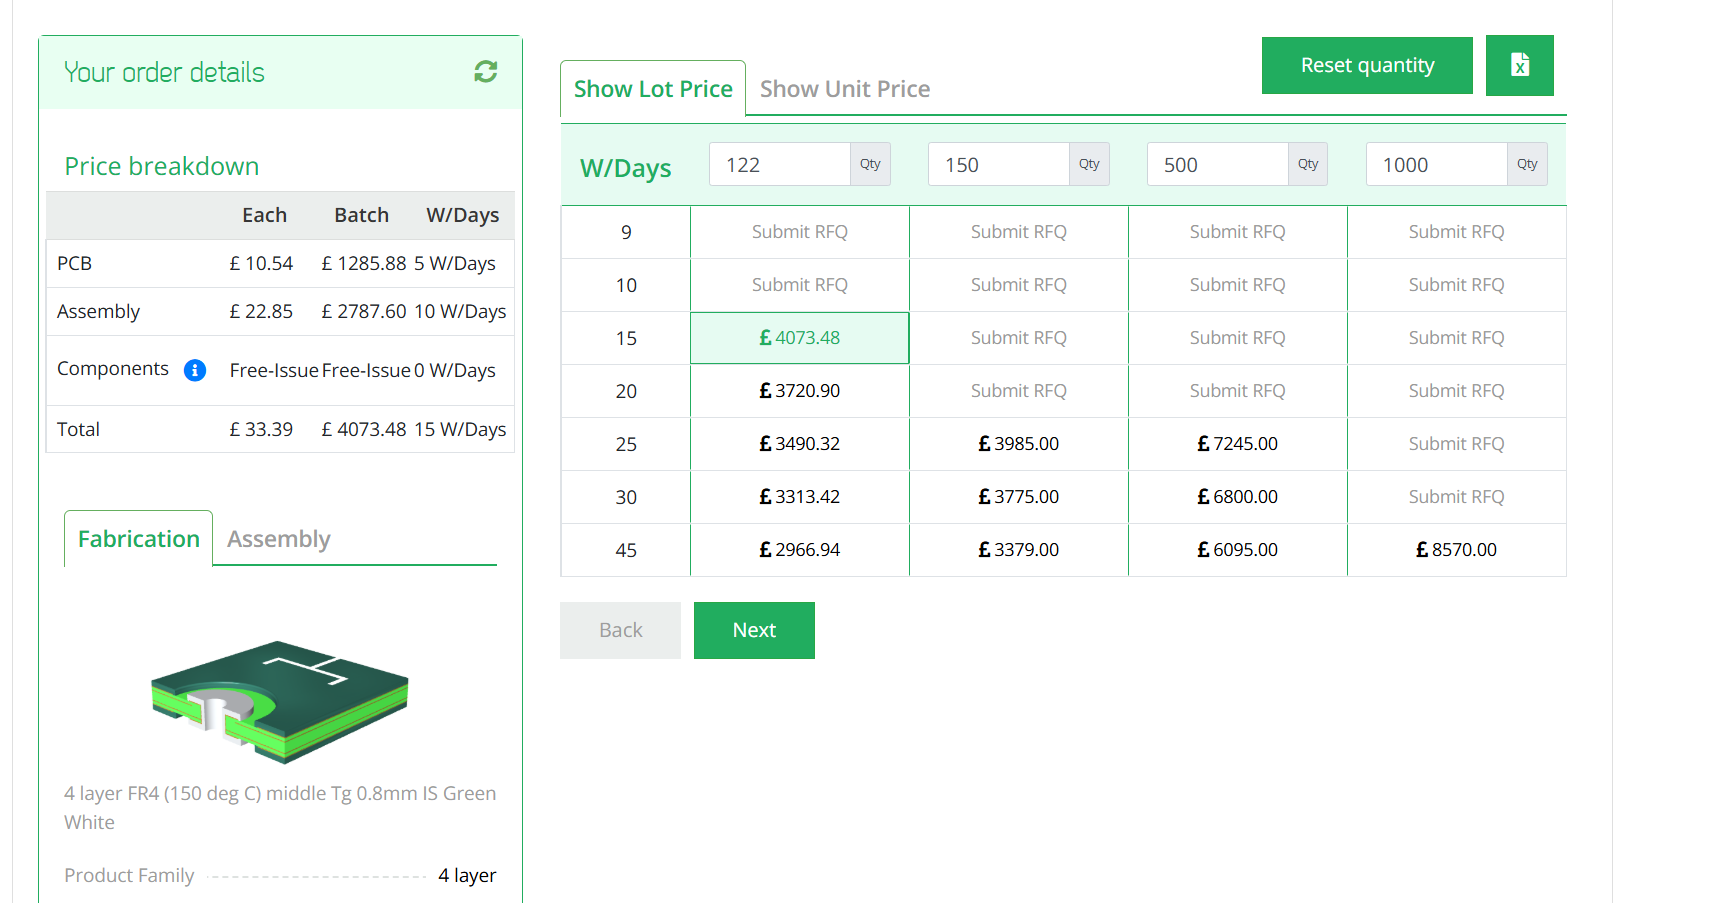
\includegraphics[scale=0.5]{PCBTrainOrder.png}
\caption{PCBTrain PCB production and assembly costs\label{fig:PCBTrainOrder}}
\end{figure}


\subsection{Changes Expected from v0.9 to v1.0}

\subsubsection{LED and Switching Circuit}

There will be minimal changes to the LED and switching circuit. Changes will be made to the position of the switching devices, placing them slightly closer to each other to reduce transmission line length. The LED will likely remain as the LC LED UT-67UV365P 365nm 0805 LED, but further LED tests will be performed. This takes a short amount of time, and may lead to discovering better LEDs in the future which would be easy to swap in due to standardised footprints.

\subsubsection{LVDS-to-TTL converter}

No changes are expected to this circuit.

\subsubsection{Power supplies}

Reverse voltage bias will be removed as no difference between normal and reverse bias was observed photon output. The overcurrent protection and power enable circuit will be reworked.

\subsubsection{Connector}

No changes are expected to this.

\subsubsection{Fibre coupler}

A brand new fibre coupler will be designed due to the recent requirement changes regarding the different fibre lengths.


\section{Server Rack and Cooling}

To house the electronics for the LI systems, two 42U server racks with 800~mm depth will be used. The front of the server rack will be used for electrical connections and displays, and the reverse/internal will be used only for fibre routing. The server racks will include Uninterruptible Power Supplies (UPS) for safe power delivery and for power processing, to avoid issues with potential instabilities in the main power supply. Each rack will include an air conditioning unit to have a controlled temperature and remove humidity from the air, as the relative humidity in the air is expected to be above 70\%. Although specific tests on running the LED electronics in humid conditions have not been carried out, it is known that the optical switches for the laser calibration system requires lower humidity levels. In order to simplify things and remove the potential of humidity issues with the LED electronics,  both server racks will be air conditioned. These systems are widely available and will be chosen closer to installation.

\section{LED Monitoring}

To monitor the light output from the LEDs before attenuation by fibres and convolution with water parameters, PMTs will be placed near to the LED sources. This is a similar design to what is currently used in the Super-K UKLI system. Each LED connector will feature a second fibre to take light to a series of PMTs, which are expected to be Hamamatsu H10721-210. Due to the 8~mm diameter of the PMT window, up to 16 fibres can be attached, meaning one PMT can monitor up to 16 LED boards at once. Each PMT will be powered by a unique low cost power supply developed for the SK UKLI system. These will be housed in a small 2--3 U server rack. The signals from the PMTs will then go to the dedicated HK electronics channels that are set up for monitoring.

\section{Control System for LEDs}\label{sec:LEDcontrol}

The LEDs are driven by a differential LVDS signal originating from the FPGA. The FPGA in use is the Genesys 2 \cite{Genesys2} development board, which operates a pulsing VHDL module clocked at \SI{300}{\mega\hertz}. Pulses are generated on the rising edge of this clock, and toggling the output (i.e., asserting and then deasserting the trigger) requires a minimum of two clock cycles. Consequently, the shortest achievable pulse duration in this configuration is 3.3~ns.

One of the main limitations of this setup is the coarse time resolution: pulse durations are effectively constrained to integer multiples of \SI{3.3}{\nano\second}. To achieve a broader and more finely resolved spectrum of optical injection into the detector, improved temporal precision is necessary. This is accomplished using the Xilinx \texttt{IODELAY} primitive, originally designed for high-speed interface timing alignment. The \texttt{IODELAY} module permits fine-tuning of signal timing to account for PCB trace mismatches, and in this application, it is repurposed to introduce controlled delays between pulses.

To generate shorter pulses, two identical signals are created, one of which is delayed using \texttt{IODELAY}. These signals are then combined using a logical \texttt{AND} operation, producing a narrower pulse. Since the \texttt{IODELAY} module requires one clock cycle to process the input, both signals—regardless of whether they are delayed—must pass through an \texttt{IODELAY} stage to ensure temporal synchronisation.

Conversely, to produce longer pulses, the same methodology is applied, but the signals are combined using a logical \texttt{OR} gate instead. This approach extends the pulse width beyond the base clock resolution, enabling pulse durations ranging from approximately \SI{1.5}{\nano\second} to \SI{4.5}{\nano\second} in 49 discrete steps. The lower bound is determined by the threshold of the LVDS-to-TTL converter, which does not respond to pulses shorter than approximately \SI{1.5}{\nano\second} .

For channels using the longest optical fibres, this extended range is sufficient, given the intrinsic dispersion in the fibre optics of around \SI{5}{\nano\second}. However, shorter fibres require additional pulse shaping. To this end, an additional mechanism is implemented using a \texttt{for} loop structure within the FPGA logic. This allows the pulse to persist for multiple clock cycles, effectively producing longer pulses by repetition. However, due to FPGA architecture constraints, each iteration of the loop consumes a clock cycle, necessitating careful timing control. For instance, to produce a \SI{6.6}{\nano\second} pulse, the loop must be configured for two cycles, accounting for the loop overhead.

Further refinement is under investigation through the daisy-chaining of multiple \texttt{IODELAY} modules. This would enable sub-nanosecond granularity by introducing additional intermediate delay steps. While promising, this technique requires further validation and testing.

The pulse control data structure is currently under development. There are two types of pulse description considered. In the first option, the software interface would require two parameters per channel: a \textit{coarse} step and a \textit{fine} step, reflecting the approach used in the SK system. The other option would be just a single variable and then simple logic turning that variable into the \textit{coarse} and \textit{fine} step that the internal logic requires. Two hardware modules are planned: one for generating the single shortest possible pulse (to minimise latency), and another for multi-cycle pulses using programmable duration. A selection logic will assess the input and route it to the appropriate module based on the desired pulse characteristics.

Each LED channel will be controlled independently, allowing for unique pulse configurations across channels. The global trigger will be derived from the system clock, and each channel will pulse in a predefined sequence while triggered from the global trigger. This architecture also supports simultaneous pulsing of multiple channels. Should asynchronous behaviour be required, additional per-channel delay logic can be implemented. Given the five distinct fibre lengths used in the system, each channel group will also include a configurable delay offset to compensate for propagation time differences. These group delays will be calibrated and fixed, with the option of fine-tuning individual channels post-deployment if necessary.

The FPGA programming remains in active development. Inter-crate communication protocols and synchronisation are currently under integration and testing.

\section{Crate Electronics}\label{sec:crate}

\subsection{Overview}

The system specification calls for control of up to 122 LED channels, significantly exceeding the channel counts used in current systems such as Super-Kamiokande or LUX-ZEPLIN, which the previous generation of pulser boards are used for. To manage this complexity, the design prioritises ease of use, maintainability, and straightforward deployment, particularly given that the server racks will accommodate hundreds of optical fibres.

To achieve this, a system concept originally developed by ATLAS collaborators (specifically by Ashley Greenal) has been adapted. The original design utilises a Genesys 2 FPGA integrated into a half-width Verotec KM6-2 \cite{KM6-2} Eurocard-compatible crate for testing purposes. This concept has been extended to a full 19-inch rack width, enabling the integration of up to 36 pulser boards within a single crate.

Each FPGA is capable of interfacing with up to 38 pulser boards, thereby maximising the utilisation of available LVDS differential pairs, with an additional pair reserved for the laser trigger signal. This configuration ensures full use of the Genesys 2’s I/O capacity while maintaining flexibility for future expansion.

The system architecture consists of three primary components: the Blade (\cref{blade}), Backplane (\cref{backplane}) and Eurocard (\cref{eurocard}). This modular approach ensures scalability and facilitates debugging, replacement, and upgrades. It also provides a robust foundation for managing high channel counts while maintaining signal integrity and synchronisation across the system.

\subsection{Blade}\label{blade}

The Blade is a simple, eight layer board, that has a SEAM-40-06.5-L-10-2-A-K-TR \cite{SamtecSeam} connector which is a direct fit for the Genesys 2's FMC connector. It features a PCIE 16X connector at the edge for connectivity to the Backplane. The PCIE was selected by Ashley Greenal as it is a well documented standard connector and there are a large amount of connectors available that can be bought easily. While PCIE connectors are being used, the PCIE standards for communication are not. This is a very dense PCB with all the differential tracks on it, so buried vias and multiple layers will be used. See \cref{fig:BladeWIP} for a work in progress version.

\begin{figure}[htbp]
\centering
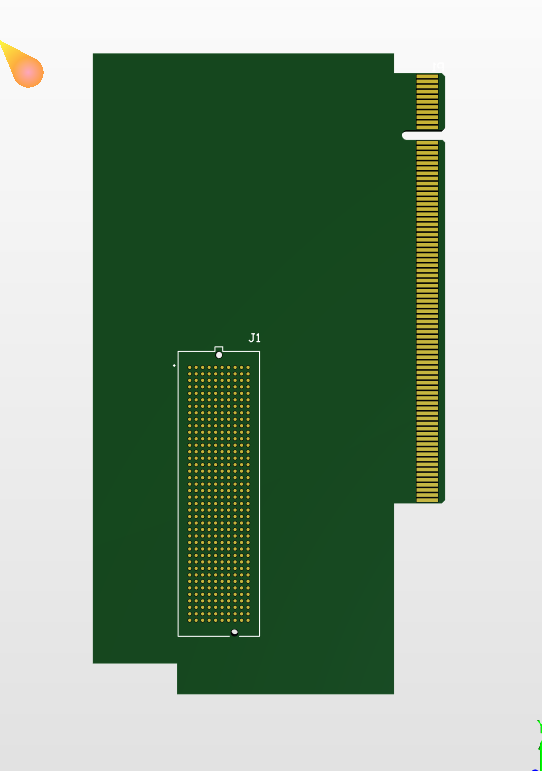
\includegraphics[scale=0.5]{G2BladeWIP.png}
\caption{Blade Work in Progress\label{fig:BladeWIP}}
\end{figure}

\subsection{Backplane}\label{backplane}

The Backplane serves two primary functions: the distribution of differential signals from the Blade to the Eurocards, and the reception and distribution of power throughout the crate system. It accepts external power inputs of \SI{12}{\volt} and \SI{\pm5}{\volt}, and includes a basic regulation circuit to stabilise these supply voltages for downstream use.

Given the mechanical constraints and routing complexity, the Backplane is implemented as a four-layer PCB with impedance-controlled traces to ensure signal integrity across all differential pairs. It features a single PCIe x16 connector to interface with the Blade, and three PCIe x8 connectors to interface with the Eurocards.

The Eurocards are positioned at slots 2, 8, and 64 within the crate. This arrangement creates two symmetrical chambers with 48 units spacing between cards, ensuring adequate space to accommodate the minimum long-term bend radius of the FP400URT optical fibres. This layout balances mechanical reliability with signal routing efficiency and supports long-term maintainability of the system. See \cref{fig:BackplaneWIP} for a work in progress version.

\begin{figure}[htbp]
\centering
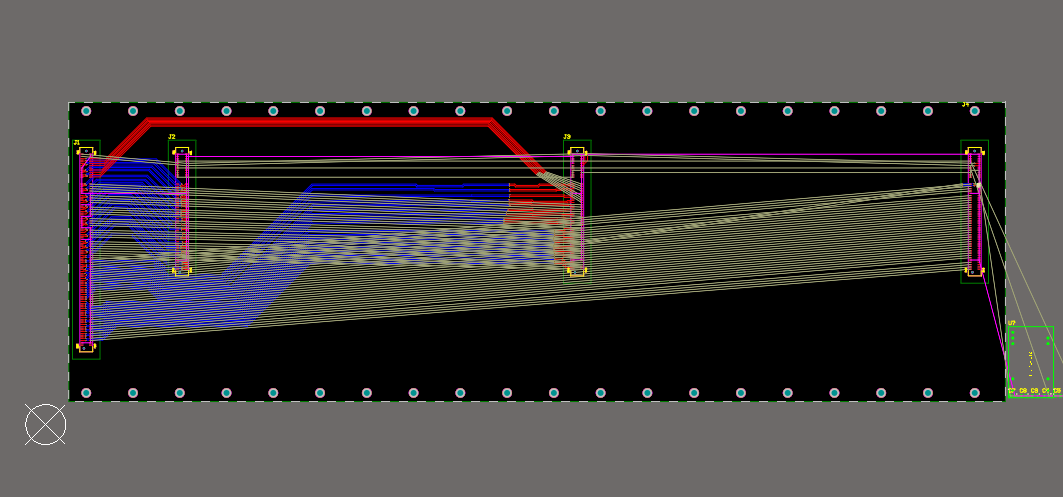
\includegraphics[scale=0.5]{BackplaneWIP.png}
\caption{Backplane Work in Progress\label{fig:BackplaneWIP}}
\end{figure}

\subsection{Eurocard}\label{eurocard}

The Eurocard format defines the physical and electrical standard for the crate system, hence the naming convention. Each Eurocard is equipped with a PCIe x8 connector for interfacing with the Backplane, and is designed to host up to 18 pulser boards—nine mounted on each face. Pulser boards connect via FS-1332120 Male\cite{1332120} connectors, and each socket includes two mounting holes for mechanical standoffs.

The board layout on each side consists of two staggered rows: five sockets in the back row and four in the front. The two faces are laterally offset by approximately \SI{10}{\milli\metre} to prevent interference or fibre clashes when the system is fully populated and enclosed within the crate chamber. This offset ensures smooth fibre routing and accommodates the bend radius requirements of FP400URT fibres.

Power distribution within each Eurocard is handled by a THD 12-1212 \cite{THD121212}\SI{12}{\volt} DC-DC regulator. This regulator provides local power isolation for the pulser boards and includes a control pin connected to a PCA9698 \cite{PCA9698} 40-pin GPIO expander. This allows for system-level control, enabling or disabling all pulser boards on a card—an essential feature during power-up, especially when the FPGA may inadvertently drive all differential outputs high during reprogramming.

The GPIO expander is responsible for enabling the local \SI{12}{\volt} regulator and for selectively powering individual pulser boards. This facilitates fault isolation and power savings in channels that are inactive or disconnected. Additional GPIO pins are assigned to monitor output voltage levels via the overcurrent sensing circuitry.

To provide per-channel LED power control, an AD5673 \cite{AD5673} DAC is included. It outputs analogue control voltages to the onboard adjustable regulators on each pulser board, allowing for independent LED drive voltage per channel. Both the GPIO and DAC devices communicate with the system over the I\textsuperscript{2}C protocol.

For laser synchronisation, the Eurocard includes a differential-to-NIM conversion stage. This consists of an LVDS-to-TTL converter identical to that used on the pulser boards, followed by a TTL-to-NIM converter. This ensures compatibility with legacy NIM-based timing systems used in external laser triggering. See \cref{fig:EurocardWIP} for a work in progress version.

\begin{figure}[htbp]
\centering
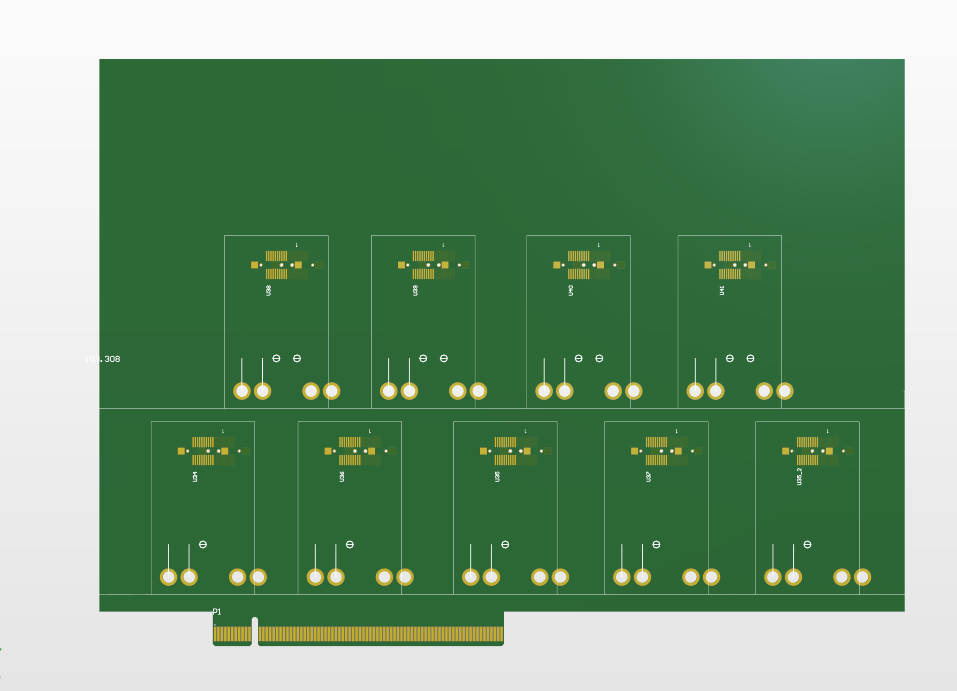
\includegraphics[scale=0.5]{EurocardWIP.png}
\caption{Eurocard Work in Progress\label{fig:EurocardWIP}}
\end{figure}




\section{Conclusions}

Write this



\appendix




% Bibliography

%% [A] Recommended: using JHEP.bst file
%% \bibliographystyle{JHEP}
%% \bibliography{biblio.bib}

%% or
%% [B] Manual formatting (see below)
%% (i) We suggest to always provide author, title and journal data or doi:
%% in short all the informations that clearly identify a document.
%% (ii) please avoid comments such as "For a review'', "For some examples",
%% "and references therein" or move them in the text. In general, please leave only references in the bibliography and move all
%% accessory text in footnotes.
%% (iii) Also, please have only one work for each \bibitem.

\printbibliography

\end{document}
